\section{Satisfacción de pasajeros de aerolíneas}

\subsection{Descripción del proyecto}

\subsubsection{Objetivo}

El objetivo es predecir la satisfacción de los pasajeros de una aerolínea en función de diversas características del pasajero y valoraciones de los servicios de vuelo. Las conclusiones de este análisis intentan ayudar a conocer los factores que más influyen a la satisfacción o insatisfacción de los pasajeros, permitiendo a la aerolínea priorizar mejoras en sus servicios.

% ---------------------------------------------------------------------------------------------------------- %

\subsubsection{Datos}

El conjunto de datos que usamos para entrenar nuestro modelo está disponible en la base de datos de Kaggle: 
\href{https://www.kaggle.com/datasets/nabihazahid/spotify-dataset-for-churn-analysis/data}{Spotify Analysis Dataset 2025}. Ya hemos descargado el fichero con extensión \texttt{.csv} en el directorio \texttt{datasets}.
En el \textit{dataset} encontramos 25 columnas, donde \code{satisfaction} es la variable objetivo, y puede tomar dos valores:
\begin{itemize}
    \item \code{satisfied}, cuando el pasajero está satisfecho; o
    \item \code{neutral or dissatisfied}, en otro caso.
\end{itemize}

En el \textit{dataset} podemos encontrar una amplia variedad de atributos que incluyen:

\begin{itemize}

    \item \code{Column0}: De tipo entero. Número identificativo de la fila.

    \item \code{id}: De tipo entero. Número identificativo del pasajero.

    \item \code{Gender}: De tipo categórico. Género del pasajero. 

    \item \code{Customer Type}: De tipo categórico. Tipo de cliente (leal o desleal).

    \item \code{Age}: De tipo entero. Edad del cliente.

    \item \code{Type of Travel}: De tipo categórico. Tipo de viaje (viaje personal o por negocios).

    \item \code{Class}: De tipo categórico. Clase del viaje (\textit{Eco}, \textit{Eco Plus} o \textit{Business}).

    \item \code{Flight distance}: De tipo entero. Distancia de vuelo en millas.

    \item Una serie de atributos referidos a valoraciones de servicio: De tipo entero. Todos los valores en una escala de 0 a 5. Estos atributos son \code{Inflight wifi service}, \code{Departure/Arrival time convenient}, \code{Ease of Online booking}, \code{Gate location}, \code{Food and drink}, entre otros.

    \item \code{Departure Delay in Minutes}: De tipo entero. Minutos de retraso en la salida.

    \item \code{Arrival Delay in Minutes}: De tipo entero. Minutos de retraso en la llegada.
    
\end{itemize}

% ---------------------------------------------------------------------------------------------------------- %
% ---------------------------------------------------------------------------------------------------------- %
% ---------------------------------------------------------------------------------------------------------- %

\subsection{Exploración y preprocesado de datos}

\subsubsection{Carga de datos}

La carga de datos la realizamos de nuevo con el nodo <<CSV Reader>>. En la Figura \ref{fig:passenger_satisfaction_CSV_reader} vemos que el conjunto de datos tiene 25 976 ejemplos, cada uno con 25 columnas.

Como en el anterior problema, eliminamos las columnas \code{Column0} e \code{id}, ya que no aportan capacidad discriminativa de la clase.  

\begin{figure}[h!]
    \centering
    \fbox{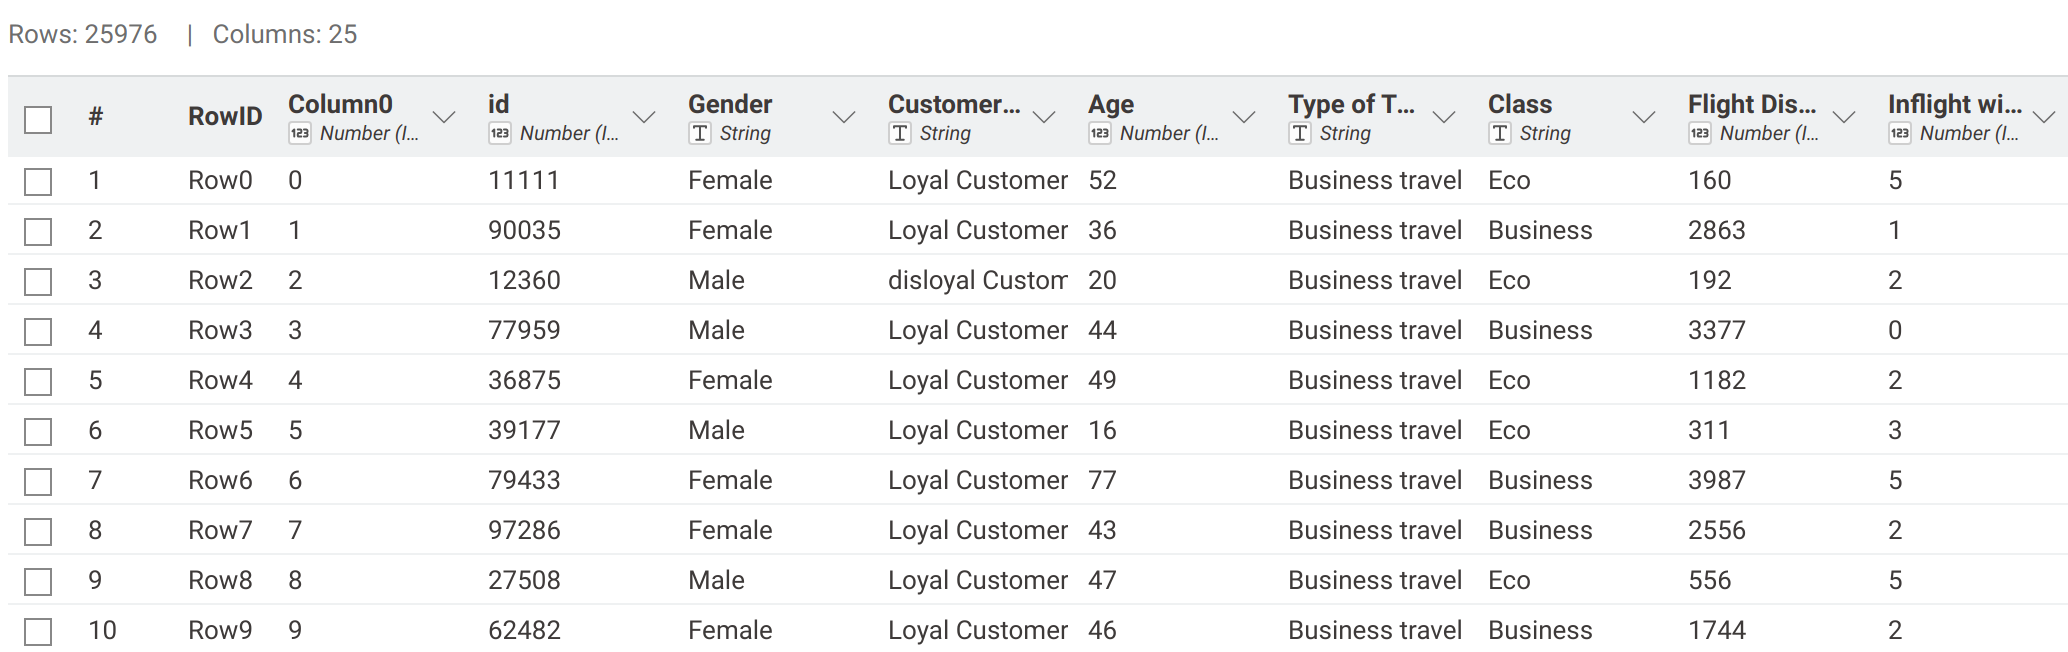
\includegraphics[width=1.0\textwidth, keepaspectratio]{secciones/sec3/imagenes/passenger_satisfaction_CSV_reader.png}}
    \caption{
        Visualización de los datos en crudo del segundo problema. 
        Obtenido del nodo <<CSV Reader>>.
    }
    \label{fig:passenger_satisfaction_CSV_reader}
\end{figure}

Se comprueba que no existen filas duplicadas en el \textit{dataset}.

% ---------------------------------------------------------------------------------------------------------- %

\subsubsection{Análisis de variables}

\paragraph*{Variables categóricas.}

En la Figura \ref{fig:passenger_satisfaction_statistics_categorical_variables} se observa la tabla de estadísticas principales de las variables categóricas. De ella, podemos extraer la siguiente información:

\begin{itemize}

    \item \code{Gender}: Atributo con dos categorías posibles, y estas están bastante equilibradas (50.71\% de mujeres frente al 49.29\% de hombres).
    
    \item \code{Customer Type}: Atributo que presenta dos categorías, siendo la mayoritaria \code{Loyal customer}, que representa el 81.53\% de las instancias, mientras que \code{disloyal customer} corresponde al porcentaje restante.
    
    \item \code{Type of Travel}: Atributo con dos categorías; el 69.44\% de las instancias corresponden a \code{Business travel}, y el 30.56\% restante a \code{Personal travel}.

    \item \code{Class}: Atributo con tres categorías, donde \code{Business} predomina con un 48.1\% de las instancias, seguida por \code{Eco} con un 44.52\%, y finalmente \code{Eco Plus} con el porcentaje restante.
    
    \item \code{Satisfaction}: Variable objetivo. El 56.1\% de las instancias tienen etiqueta \code{neutral or dissatisfied}, mientras que el 43.9\% restante corresponde a \code{satisfied}.
    
\end{itemize}

\begin{figure}[h!]
    \centering
    \fbox{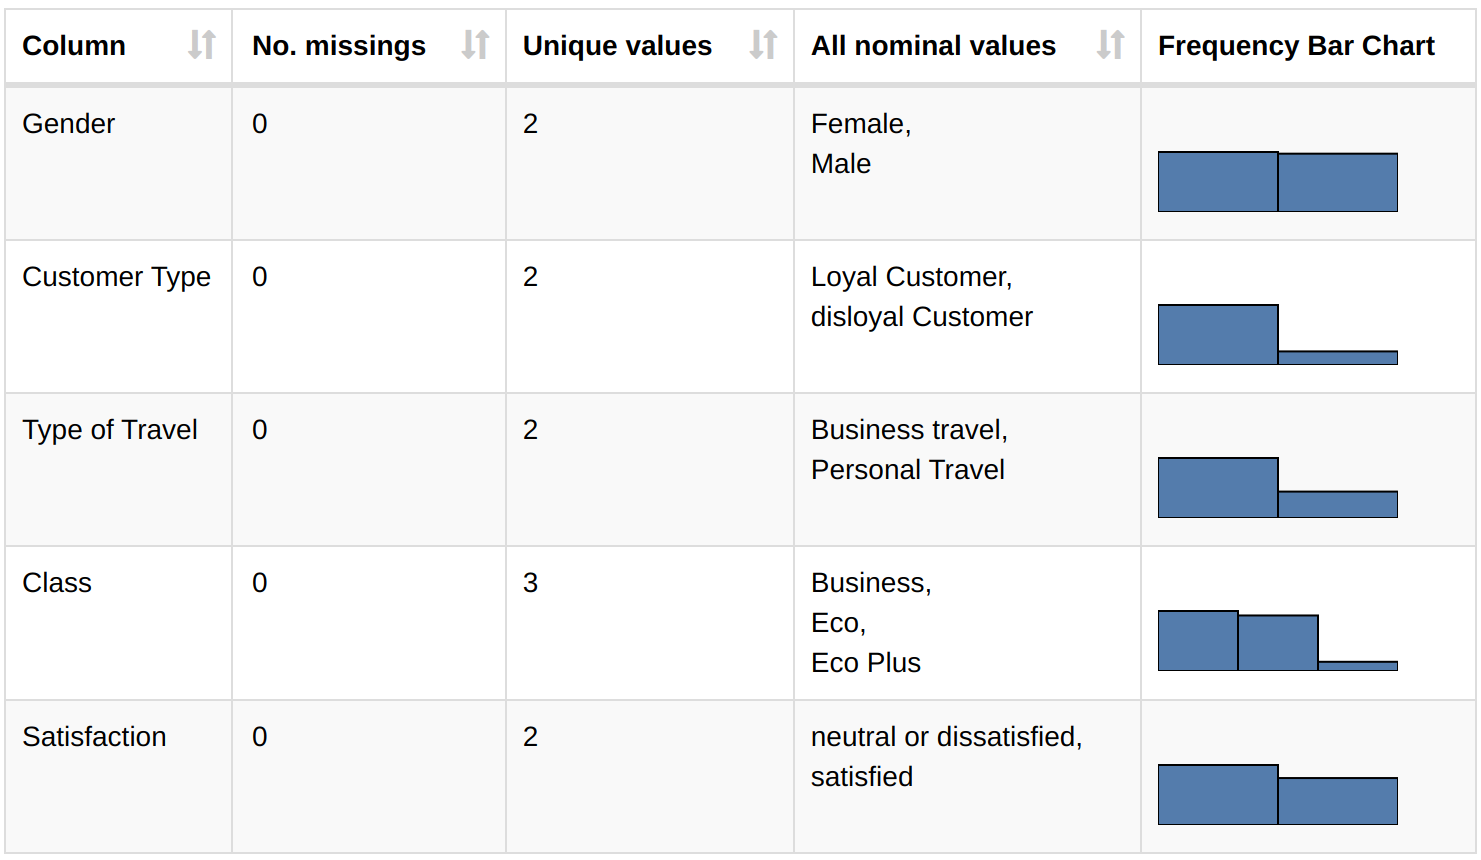
\includegraphics[width=0.85\textwidth, keepaspectratio]{secciones/sec3/imagenes/passenger_satisfaction_statistics_categorical_variables.png}}
    \caption{
        Visualización del análisis exploratorio de variables categóricas. 
        Obtenido del nodo <<Data Explorer>> de la extensión \textit{KNIME JavaScript Views (Labs)}.
    }
    \label{fig:passenger_satisfaction_statistics_categorical_variables}
\end{figure}

Cabe destacar que ninguna de estas variables presenta valores faltantes.

¿Cómo se relacionan estos atributos entre sí y con la variable objetivo? Las Figuras \ref{fig:passenger_satisfaction_parallelcategories_variables} y \ref{fig:passenger_satisfaction_statistics_categorical_variables} tratan de mostrar las relaciones y patrones de asociación entre las variables categóricas, así como su posible vínculo con el nivel de satisfacción de los pasajeros. En particular, la primera figura ilustra visualmente cómo las categorías se conectan entre sí mediante un gráfico de categorías paralelas, mientras que la segunda presenta una matriz de asociación que cuantifica la fuerza de las relaciones entre pares de variables. 

Aquí podemos identificar los siguientes aspectos destacados:

\begin{figure}[h!]
    \centering
    \fbox{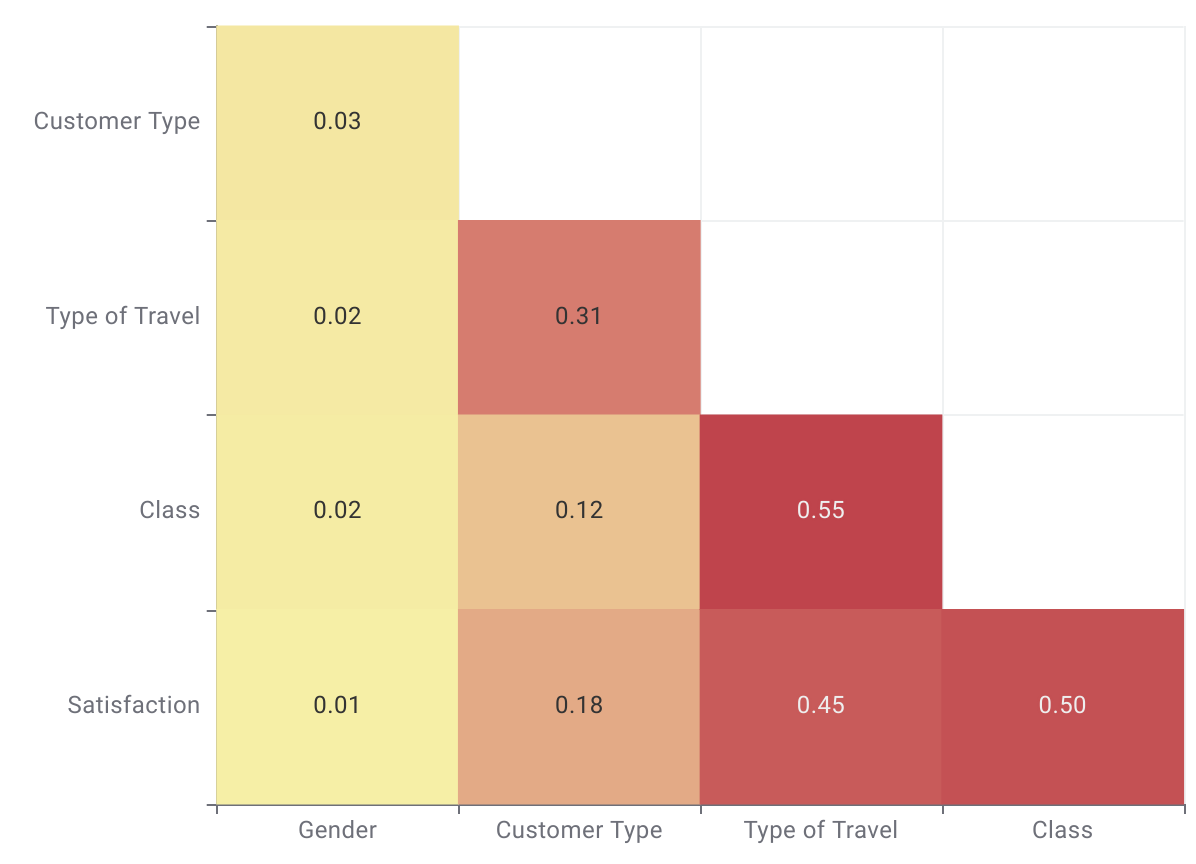
\includegraphics[width=0.7\textwidth, keepaspectratio]{secciones/sec3/imagenes/passenger_satisfaction_corrmatrix_categorical.png}}
    \caption{
        Matriz de asociación (basada en el valor chi-cuadrado de Pearson, normalizado mediante el coeficiente V de Cramer) entre variables categóricas. Obtenido de un componente creado propio, <<Association Matrix>>, que calcula las asociaciones entre cada par de variables (mediante el nodo <<Linear Correlation>>) y las plasma en un mapa de calor.
    }
    \label{fig:passenger_satisfaction_corrmatrix_categorical}
\end{figure} 

\begin{figure}[h!]
    \centering
    \fbox{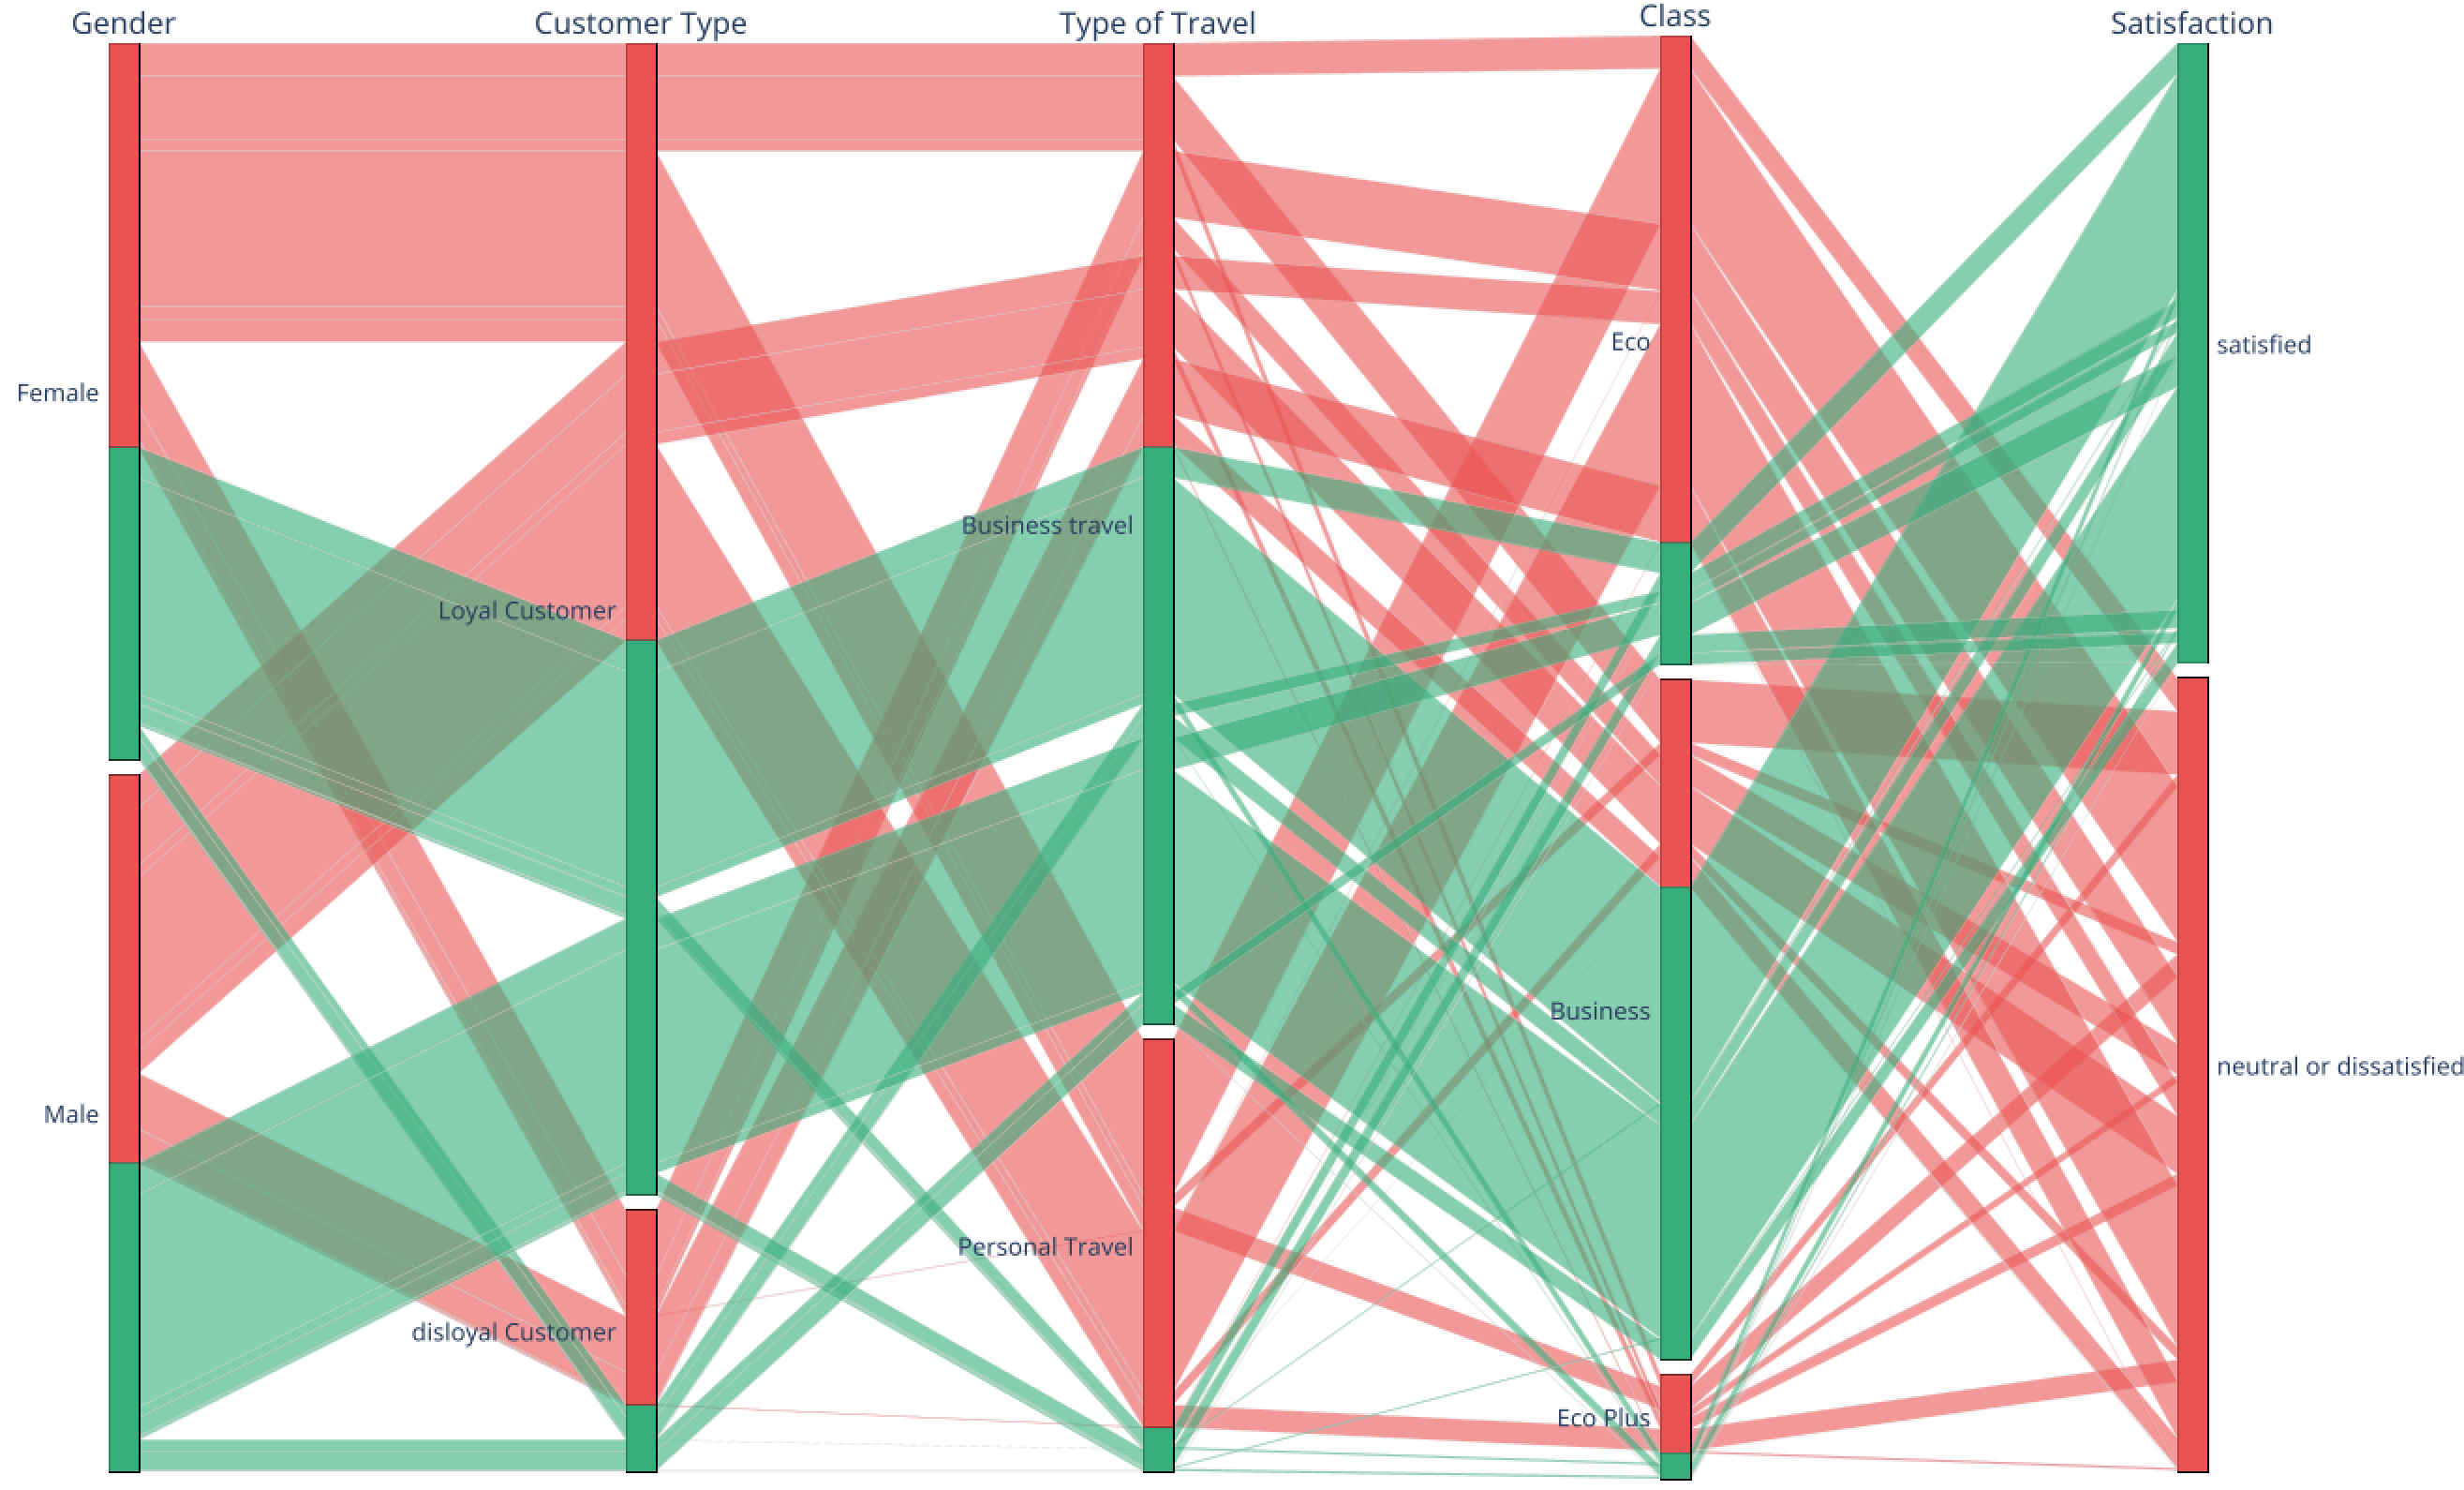
\includegraphics[width=\textwidth, keepaspectratio]{secciones/sec3/imagenes/passenger_satisfaction_parallelcategories_variables.png}}
    \caption{
        Visualización de categorías paralelas en las variables categóricas.
    }
    \label{fig:passenger_satisfaction_parallelcategories_variables}
\end{figure} 

\begin{itemize}

    \item El atributo \code{Gender} no muestra asociación significativa con otros atributos categóricos ni con la variable objetivo.

    \item El resto de atributos categóricos sí presentan cierto nivel de asociación con la variable objetivo. En el gráfico de categorías paralelas se observa que los pasajeros \code{disloyal}, aquellos que realizan \code{personal travel} y los que viajan en clase \code{Eco} o \code{Eco Plus}, tienden a mostrar un nivel de satisfacción significativamente menor en comparación con el resto de grupos.

    \item Se aprecia una fuerte asociación entre \code{Class} y \code{Type of Travel}, dado que la mayoría de los pasajeros que viajan por motivos de negocio lo hacen en clase \code{Business}, lo cual resulta coherente con las expectativas del contexto.

    \item También se identifica ---con menor intensidad--- una relación relevante entre \code{Customer Type} y \code{Type of Travel}, ya que la totalidad de los pasajeros clasificados como \code{disloyal} realizan viajes de negocios, si bien no al contrario: la mayoría de viajes por negocios son leales. 

\end{itemize}

A diferencia del problema anterior, en este caso sí se identifican patrones discriminativos más definidos entre las variables, los cuales permiten distinguir con mayor claridad los distintos niveles de la variable objetivo. Estos patrones se ven aún más reforzados gracias al mayor volumen de datos disponible. 


\paragraph*{Variables numéricas.}

La Figura \ref{fig:passenger_satisfaction_statistics_numerical_variables} presenta una tabla con las principales estadísticas de algunas variables numéricas del problema. De ella, se puede extraer la siguiente información:

\begin{figure}[h!]
    \centering
    \fbox{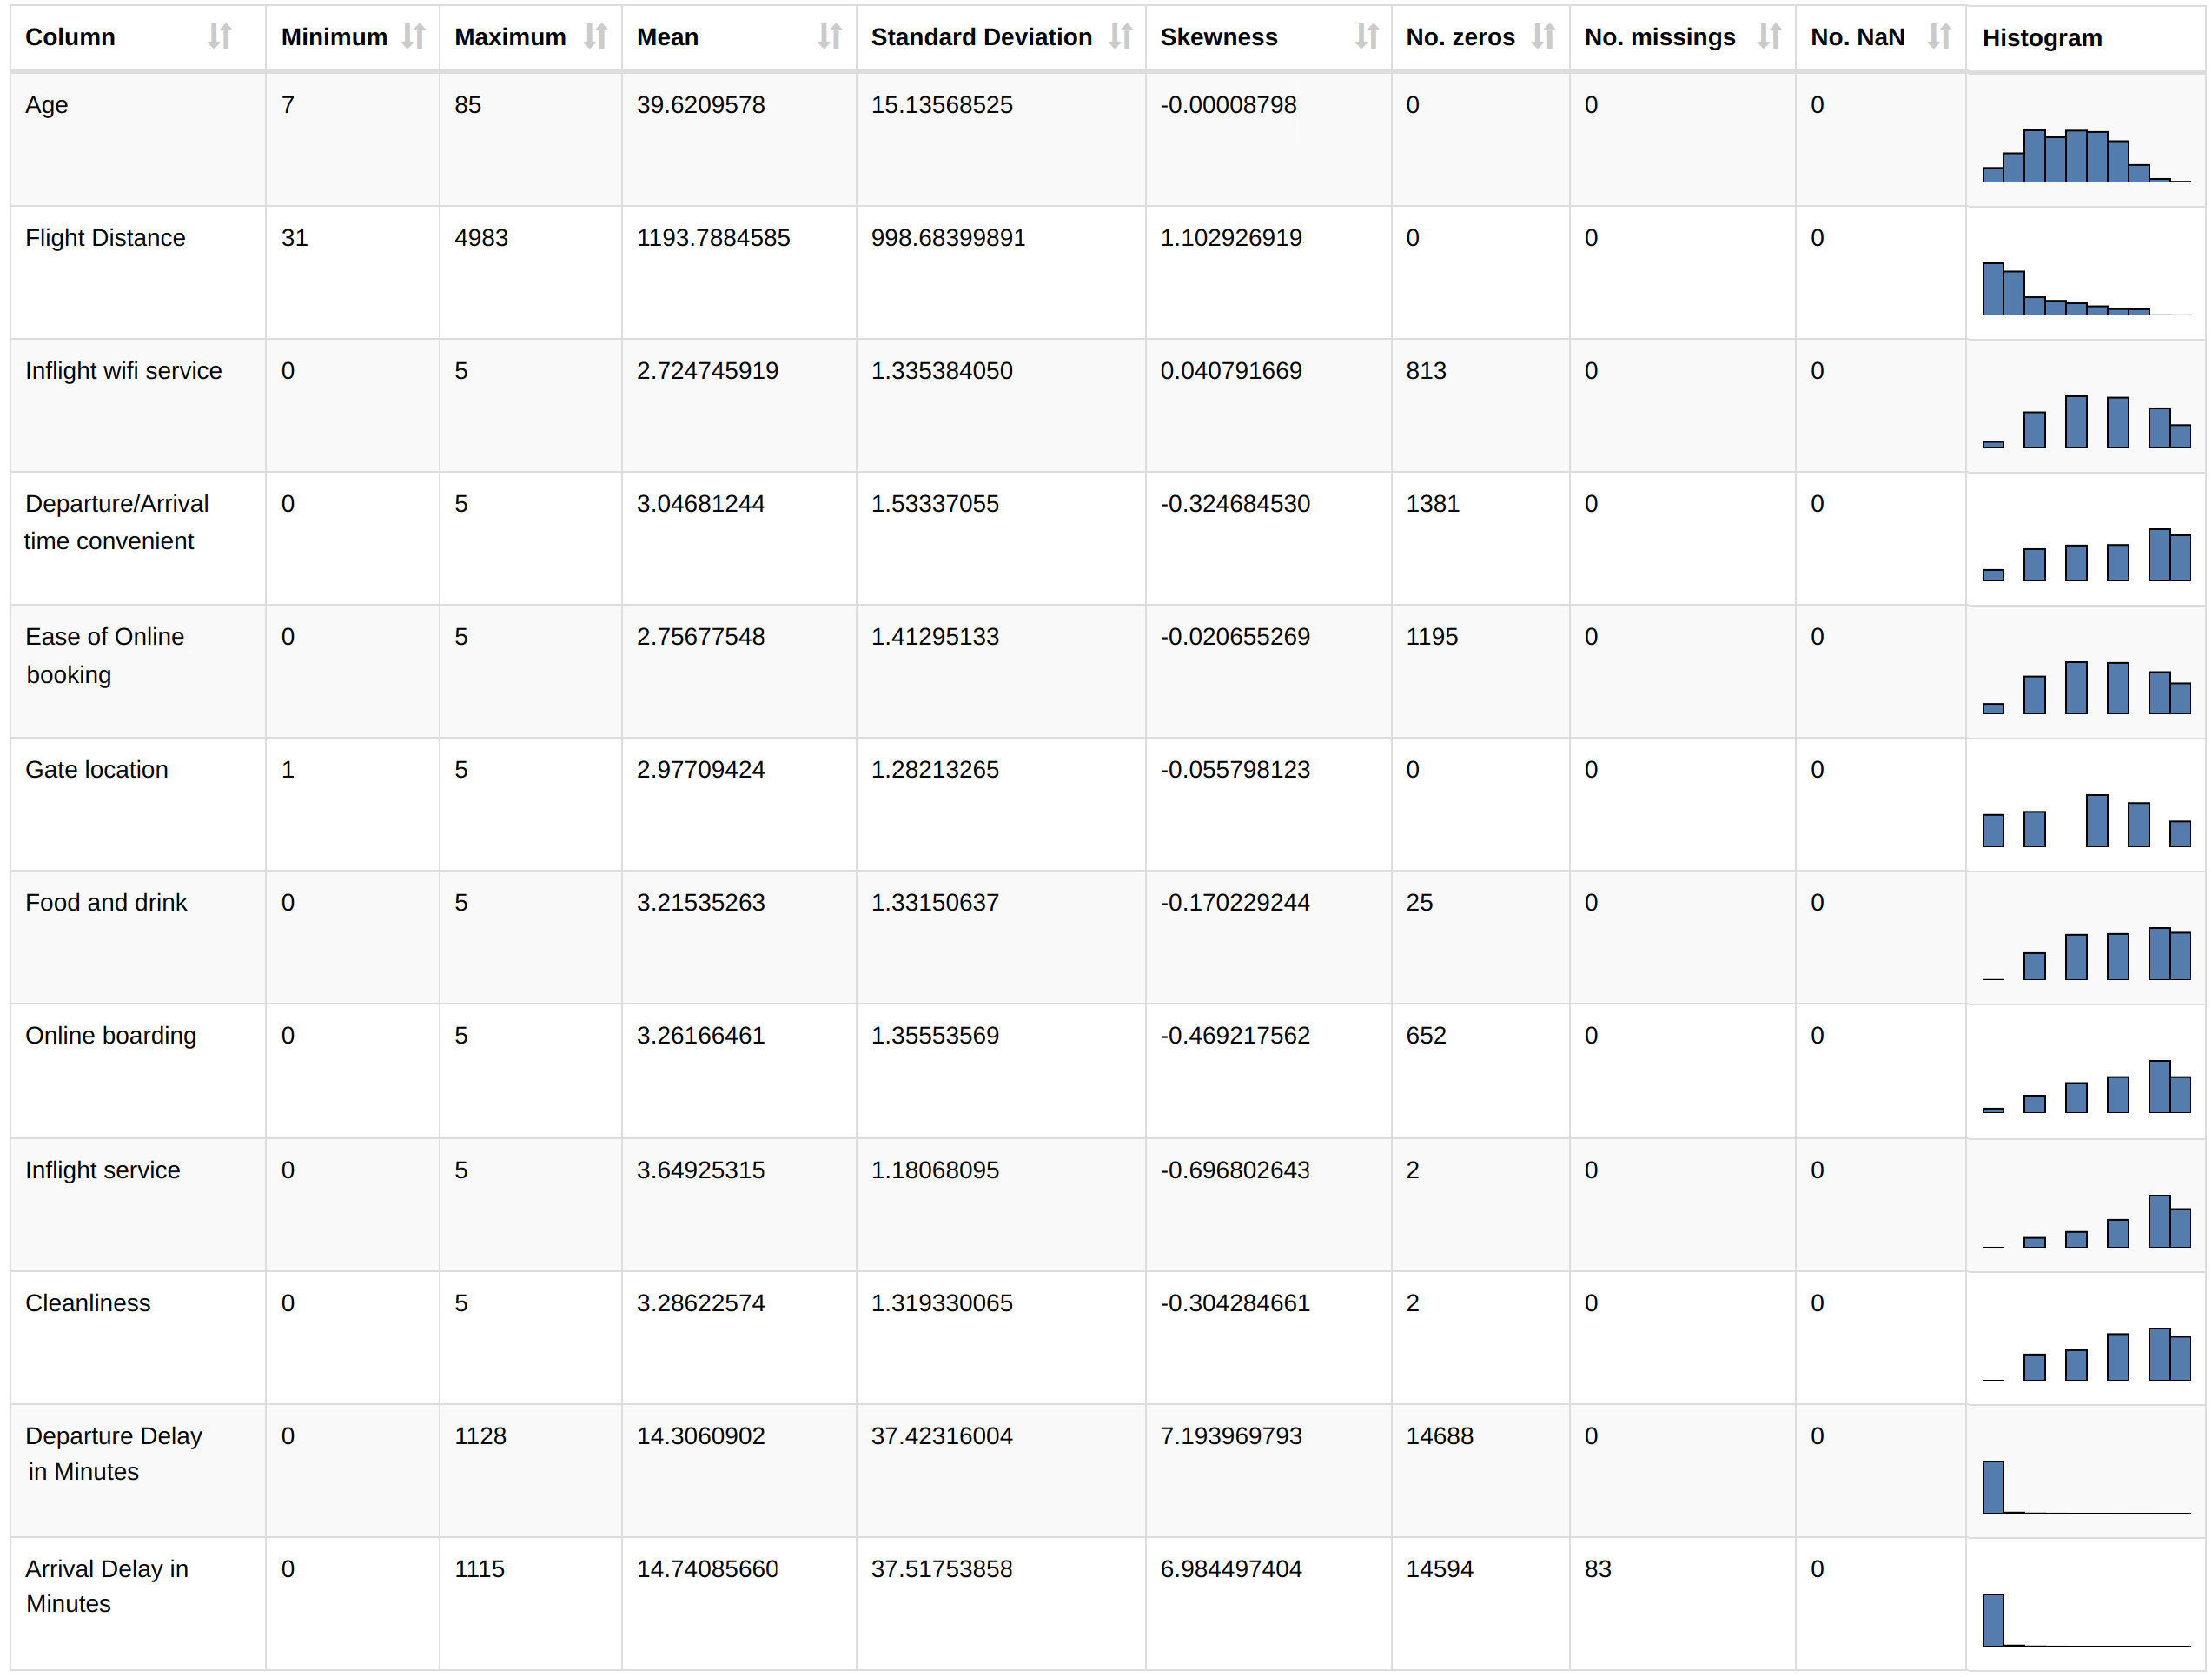
\includegraphics[width=\textwidth, keepaspectratio]{secciones/sec3/imagenes/passenger_satisfaction_statistics_numerical.png}}
    \caption{
        Visualización del análisis exploratorio de variables numéricas. 
        Obtenido del nodo <<Data Explorer>> de la extensión \textit{KNIME JavaScript Views (Labs)}.
    }
    \label{fig:passenger_satisfaction_statistics_numerical_variables}
\end{figure}

\begin{itemize}

    \item Las edades de los pasajeros (atributo \code{Age}) oscilan entre los 7 y los 85 años. La distribución parece aproximarse a una distribución normal (véase la Figura \ref{fig:passenger_satisfaction_kdeboxplot_age}), dado que presenta colas a ambos extremos y una mayor concentración de valores en torno a la media. No presenta valores extremos.
    
    \item Las distancias de los vuelos (atributo \code{Flight Distance}) muestran una distribución sesgada a la derecha (véase la Figura \ref{fig:passenger_satisfaction_kdeboxplot_flight_distance}), ya que la mayoría de los vuelos son de corta distancia, mientras que existe una cola larga hacia valores mayores correspondiente a vuelos más largos, que llegan hasta las 4000-5000 millas (apenas el 0.08\% de las instancias entran esta franja). 
    
    \item Los atributos referidos a valoraciones de servicio (como \code{Inflight wifi Service}, \code{Departure/Arrival time convenient}, \code{Food and drink}, \code{Cleanliness}, entre otros) toman valores enteros entre 0 y 5, que reflejan desde el menor hasta el mayor nivel de satisfacción percibida por los pasajeros. En general, las distribuciones de estas variables tienden a concentrarse en los valores intermedios y altos (3, 4 y 5), lo que sugiere que la mayoría de los pasajeros valoran positivamente los distintos aspectos del servicio. 
    
    \item Los retrasos en la salida y en la llegada (atributos \code{Departure Delay} y \code{Arrival Delay}, respectivamente) presentan distribuciones aún más sesgadas hacia la derecha que \code{Flight Distance} (véase la Figura \ref{fig:passenger_satisfaction_kdeboxplot_departure_delay}). La mayoría de los registros ---concretamente un 56\%--- no presentan ningún tipo de retraso (de ahí que la mediana sea 0). A medida que aumenta el tiempo de demora, la frecuencia de los casos disminuye drásticamente, lo que indica que los retrasos prolongados son mucho menos comunes y constituyen valores atípicos dentro del conjunto de datos. Cabe resaltar que \code{Arrival Delay} tiene 83 valores faltantes, de los que nos ocuparemos más tarde.

\end{itemize}

Aunque algunos atributos presentan valores atípicos, no tenemos razones para descartar las instancias, ya que estos valores son plausibles dentro del contexto del problema y reflejan situaciones reales, como retrasos excepcionales o vuelos de larga distancia. Por tanto, se consideran parte natural de la variabilidad del fenómeno estudiado y no errores de medición o registro.

\begin{figure}[h!]
    \centering
    \fbox{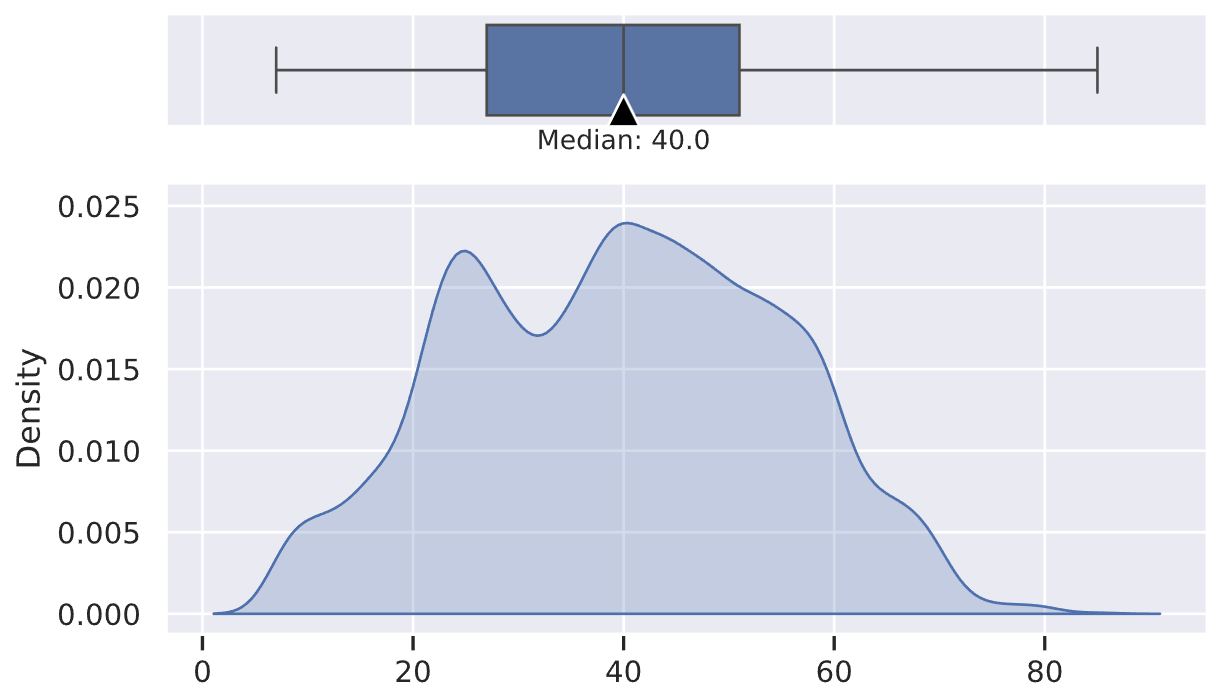
\includegraphics[width=0.7\textwidth, keepaspectratio]{secciones/sec3/imagenes/passenger_satisfaction_kdeboxplot_age.png}}
    \caption{
        Gráfica de densidad y boxplot de valores del atributo \code{Age}. 
        Obtenido de un componente creado propio, <<KDE\&Boxplot>>, que crea una imagen con un diagrama de densidad y otro de caja de una variable numérica (mediante el nodo <<Python Script>>).
    }
    \label{fig:passenger_satisfaction_kdeboxplot_age}
\end{figure}

\begin{figure}[h!]
    \centering
    \fbox{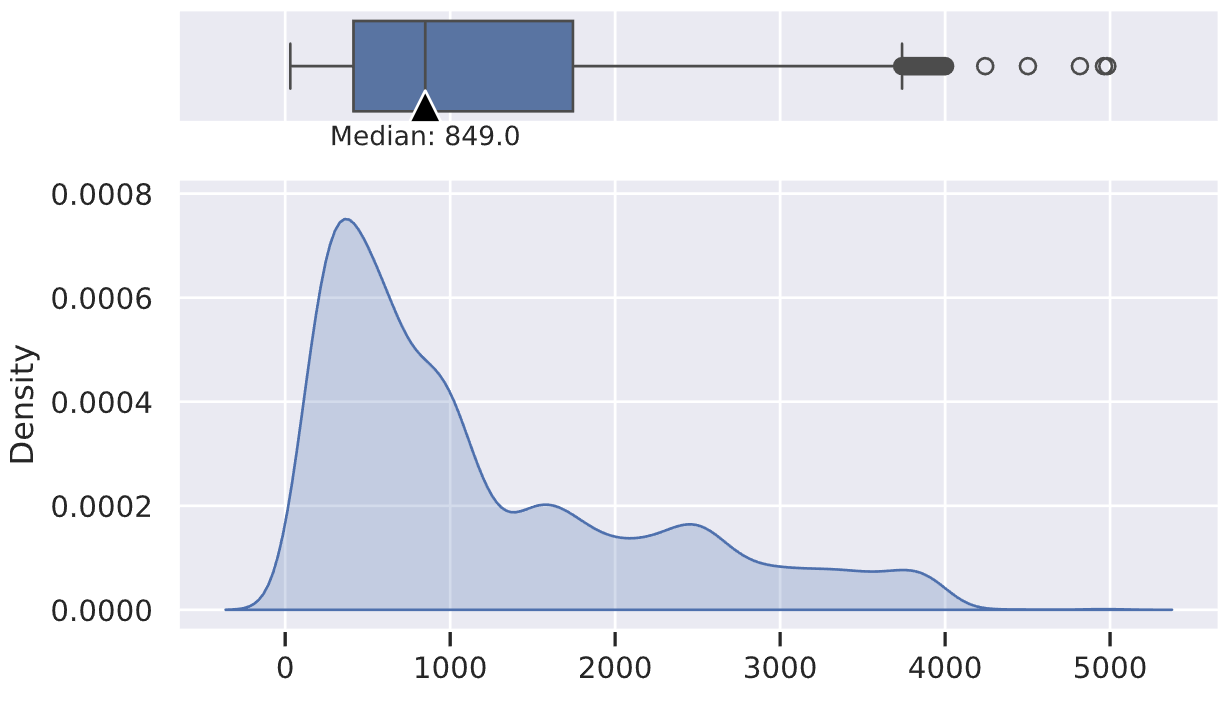
\includegraphics[width=0.7\textwidth, keepaspectratio]{secciones/sec3/imagenes/passenger_satisfaction_kdeboxplot_flight_distance.png}}
    \caption{
        Gráfica de densidad y boxplot de valores del atributo \code{Flight Distance}.
    }
    \label{fig:passenger_satisfaction_kdeboxplot_flight_distance}
\end{figure}

\begin{figure}[h!]
    \centering
    \fbox{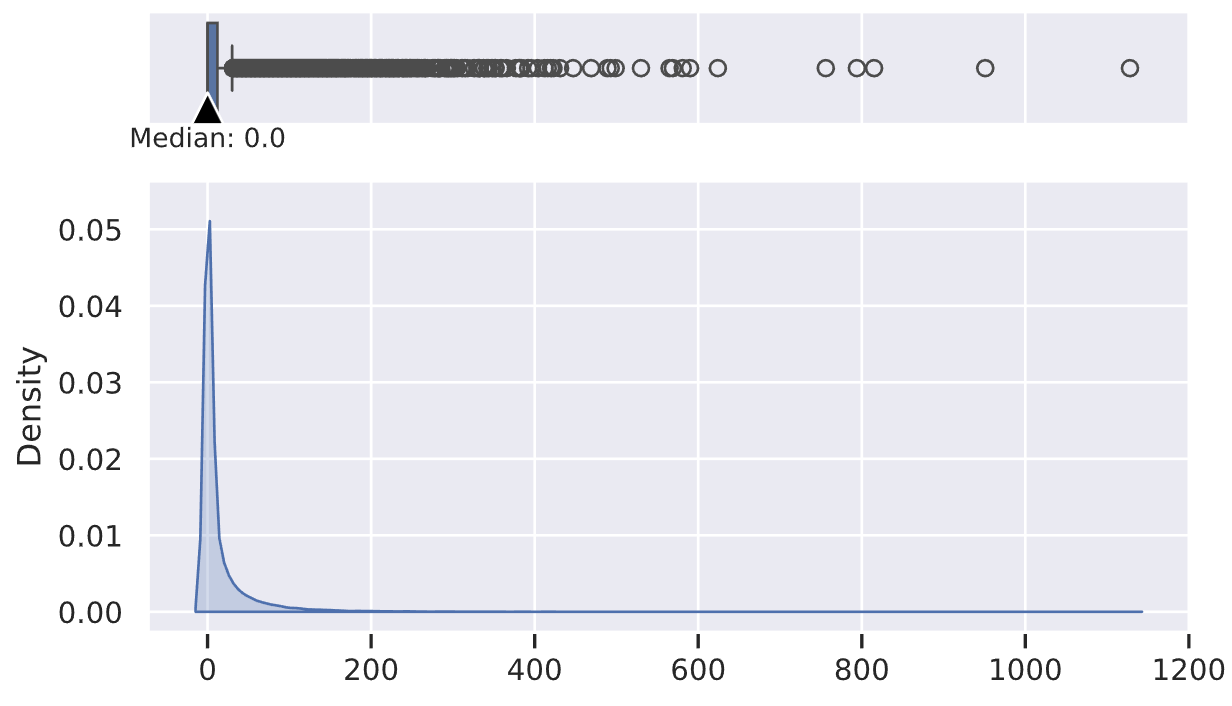
\includegraphics[width=0.7\textwidth, keepaspectratio]{secciones/sec3/imagenes/passenger_satisfaction_kdeboxplot_departure_delay.png}}
    \caption{
        Gráfica de densidad y boxplot de valores del atributo \code{Departure Delay in Minutes}.
    }
    \label{fig:passenger_satisfaction_kdeboxplot_departure_delay}
\end{figure}

Ahora veamos si existe correlación entre estas variables numéricas. La Figura \ref{fig:passenger_satisfaction_corrmatrix_numerical} muestra la matriz de correlación entre los atributos. Se puede observar un gran número de variables correlacionadas, entre las cuales se pueden reseñar:

\begin{itemize}
    
    \item \code{Departure Delay} y \code{Arrival Delay} están fuertemente correlacionadas (96\% de coeficiente de correlación de Pearson), lo que resulta lógico, ya que los retrasos en la salida suelen acumularse y provocar retrasos equivalentes en la llegada.
    
    \item Se identifican dos grupos de atributos de valoraciones de servicio que presentan correlaciones significativas dentro de cada grupo:
    
    \begin{itemize}

        \item \code{Food and drink}, \code{Cleanliness}, \code{Seat comfort} e \code{Inflight entertainment}, que podríamos asociar con la experiencia a bordo, es decir, con aspectos del confort y la calidad percibida durante el vuelo.
        
        \item \code{On-board service}, \code{Baggage handling}, \code{Inflight service}, que podríamos identificar con la calidad del servicio del personal y la atención al cliente, tanto durante el vuelo como en los procesos asociados al mismo (por ejemplo, manejo del equipaje o trato de la tripulación).
        
    \end{itemize}

    Tiene sentido que se correlacionen ya que los pasajeros podrían estar percibiendo un valor conjunto en cada grupo.

\end{itemize}

\begin{figure}[h!]
    \fbox{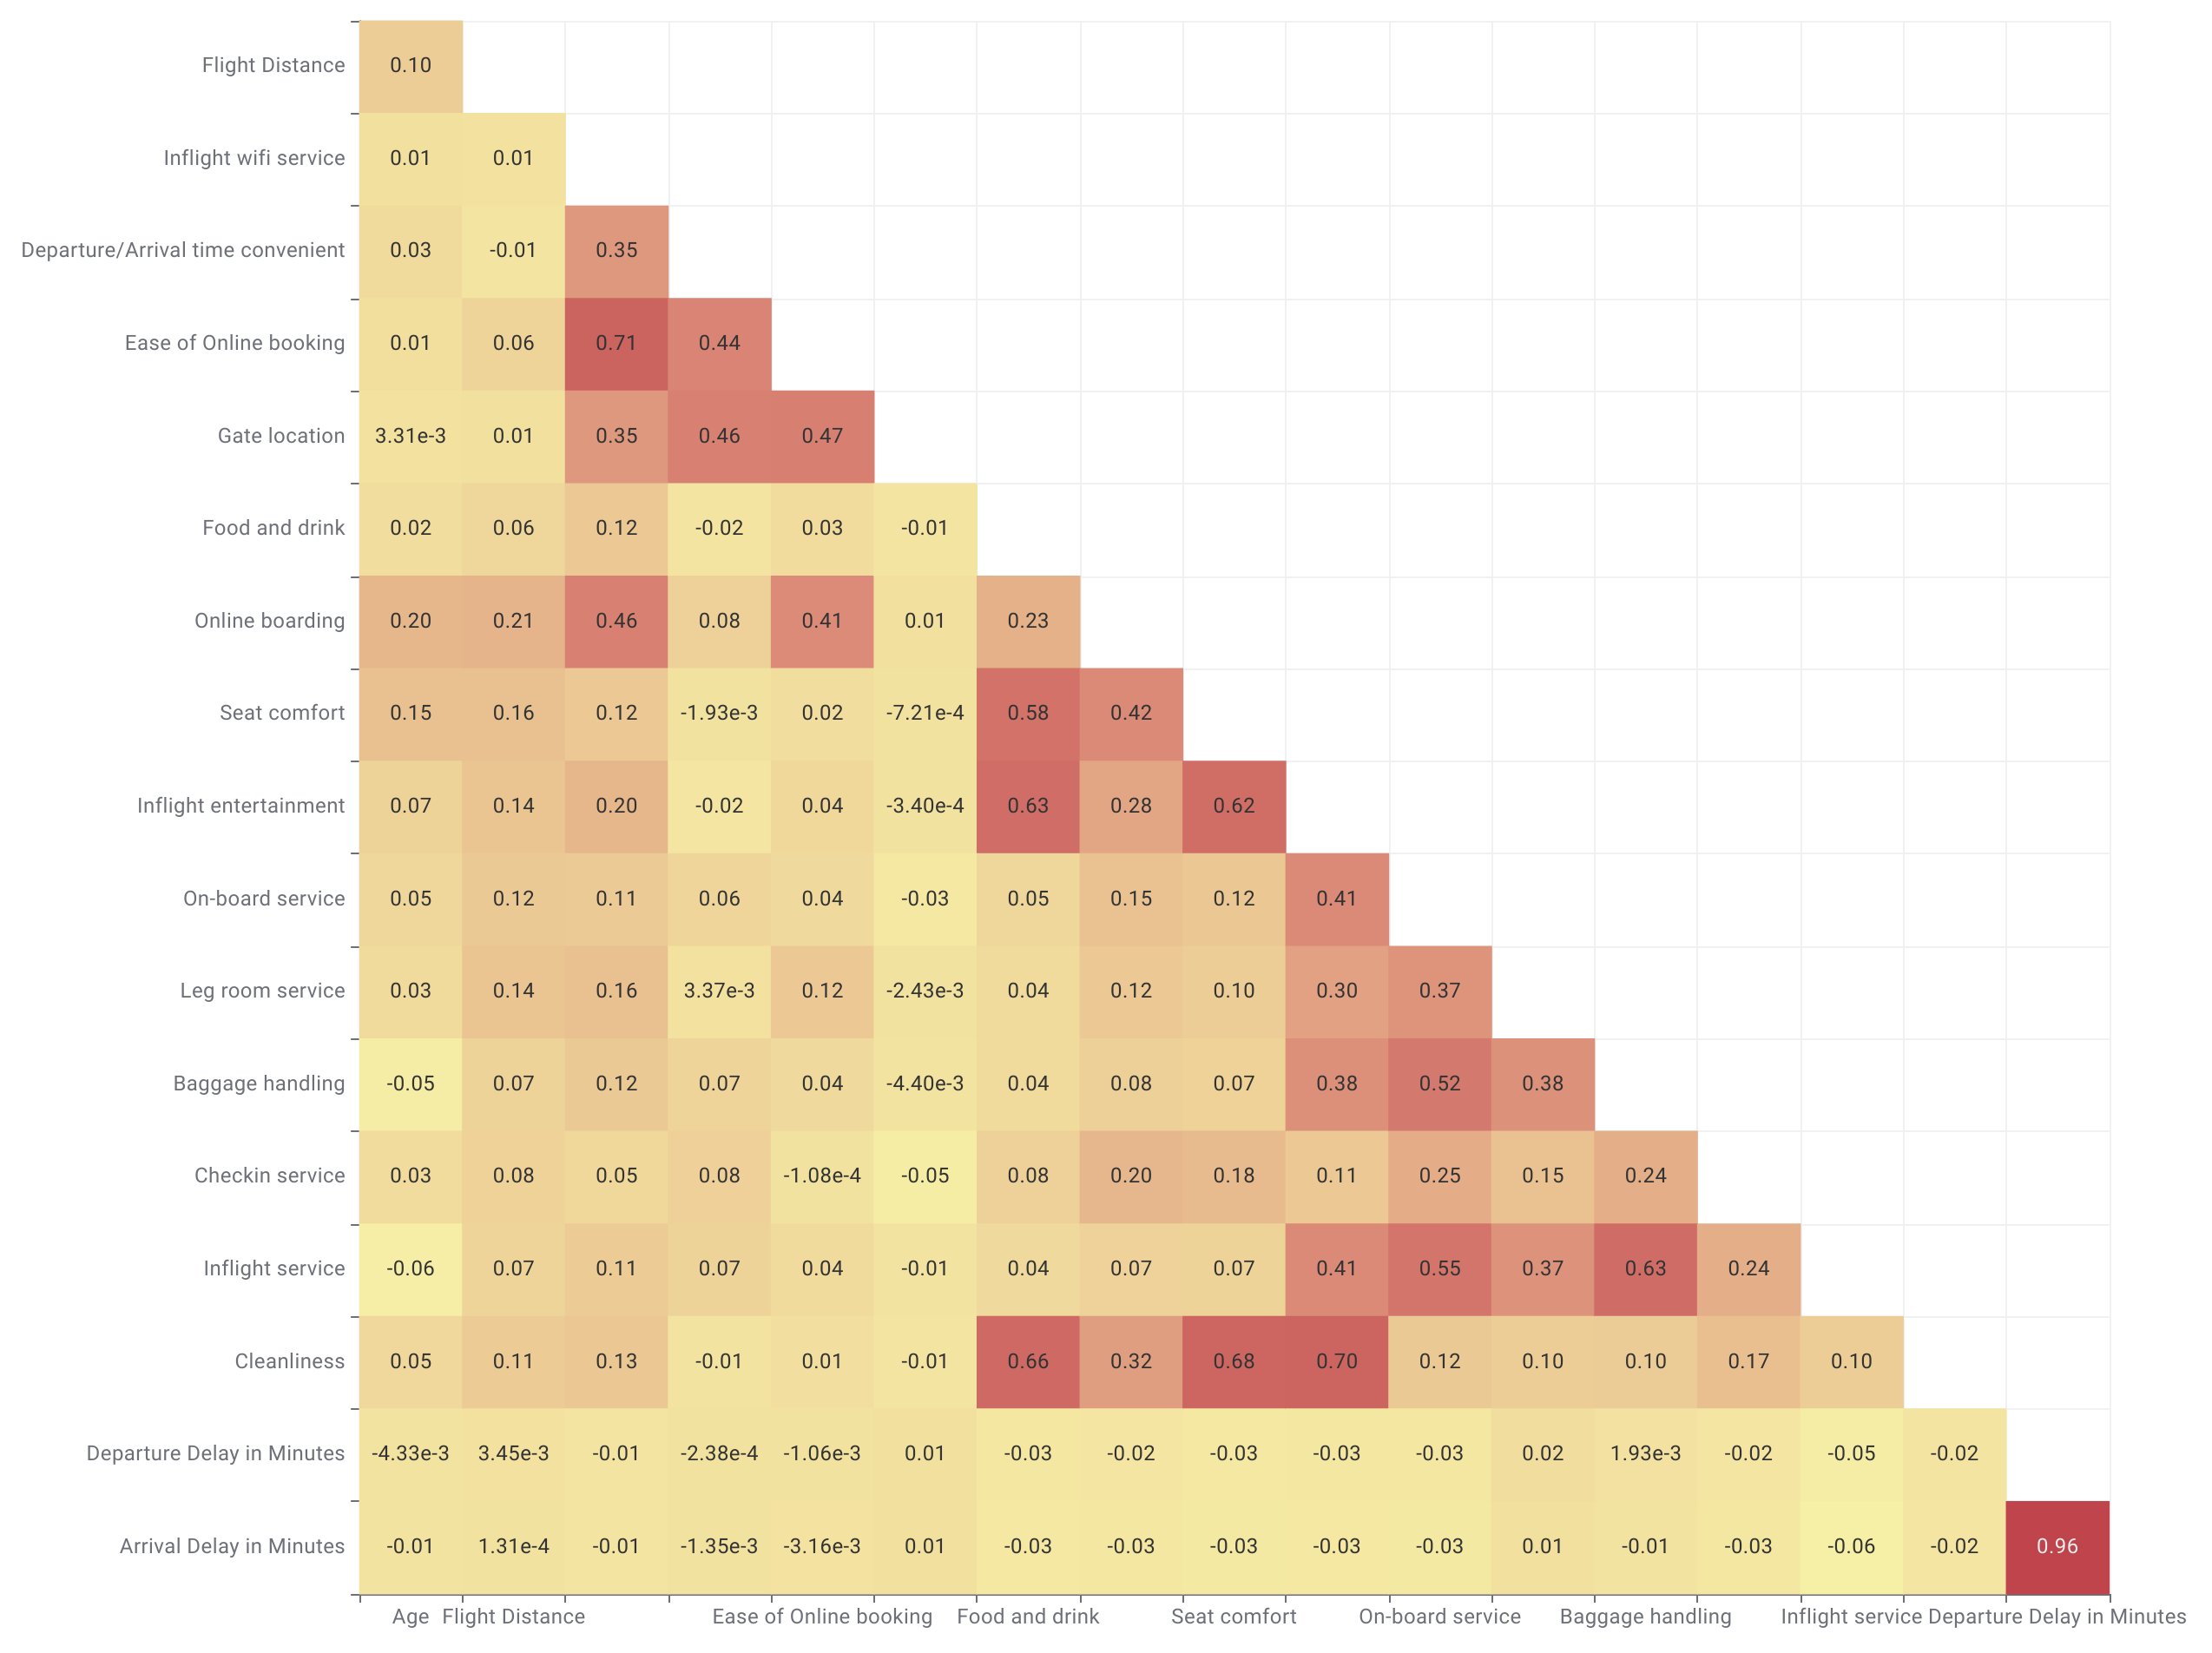
\includegraphics[width=1.0\textwidth, keepaspectratio]{secciones/sec3/imagenes/passenger_satisfaction_corrmatrix_numerical.png}}
    \caption{
        Matriz de correlación entre variables numéricas (basada en el coeficiente de correlación de Pearson). 
        Obtenido de un componente creado propio, <<Correlation Matrix>>, que calcula las correlaciones entre cada par de variables (mediante el nodo <<Linear Correlation>>) y las plasma en un mapa de calor. 
    }
    \label{fig:passenger_satisfaction_corrmatrix_numerical}
\end{figure}

Por último, al igual que se hizo en el pasado problema, se aplica la prueba $U$ de Wilcoxon-Mann-Whitney para comprobar si hay diferencias de valores entre las instancias etiquetadas en cada clase. La Figura \ref{fig:passenger_satisfaction_U_Wilcoxon-Mann-Whitney_numerical} muestra los resultados, de los que se puede destacar que prácticamente todos los \textit{p-values} son nulos, lo que indica que en todos los casos se rechaza la hipótesis nula de igualdad de distribuciones. Por tanto, se puede concluir que las variables numéricas presentan diferencias estadísticamente significativas entre los pasajeros satisfechos y los no satisfechos, lo que sugiere que dichas variables contienen información útil para la discriminación entre clases.

\begin{figure}[h!]
    \centering
    \fbox{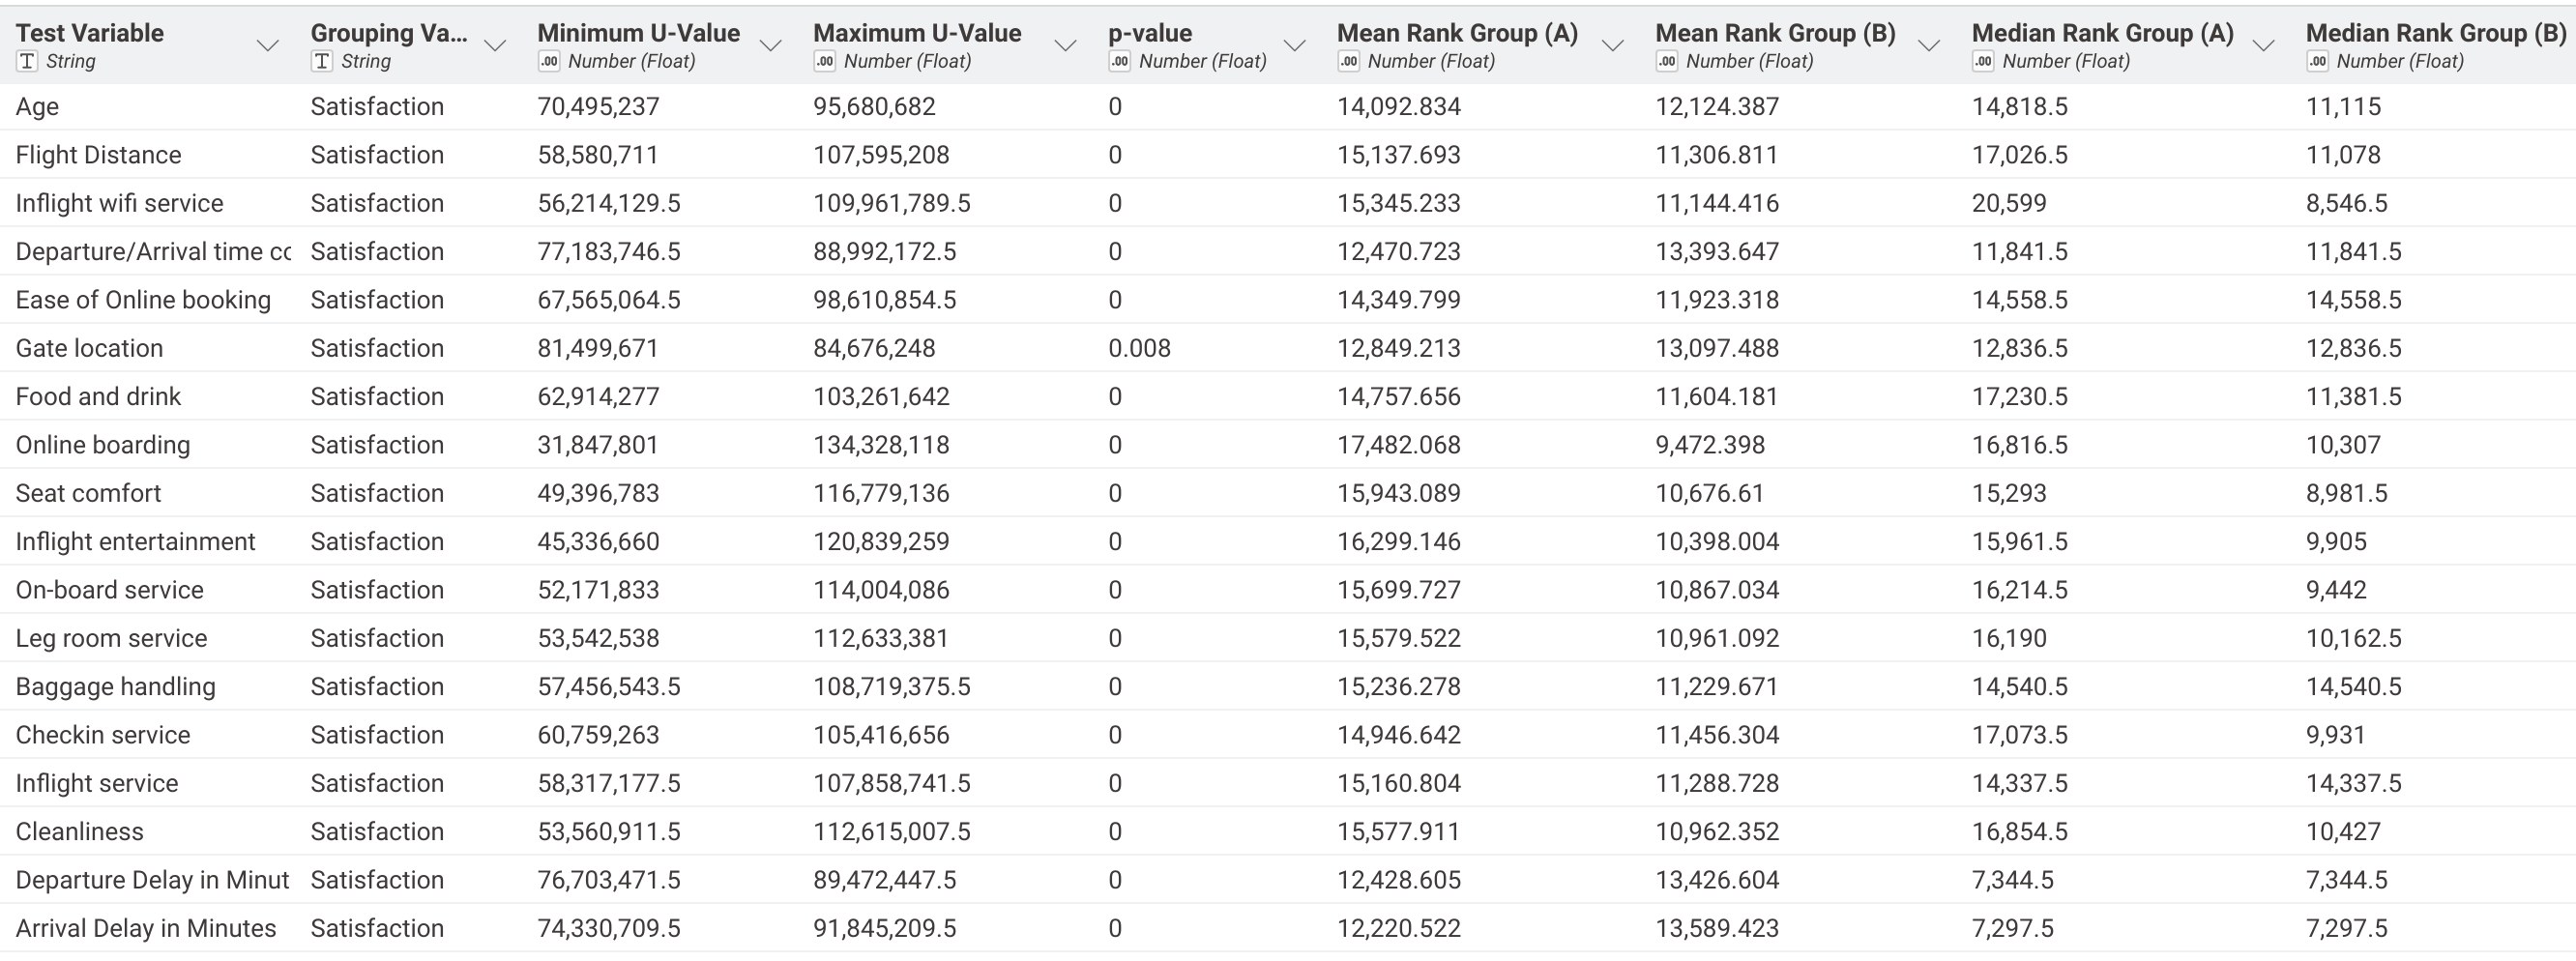
\includegraphics[width=\textwidth, keepaspectratio]{secciones/sec3/imagenes/passenger_satisfaction_mann_whitney_numerical.png}}
    \caption{
        Prueba $U$ de Wilcoxon-Mann-Whitney aplicada sobre los valores de los atributos numéricos pertenecientes a las instancias de cada categoría. 
    }
    \label{fig:passenger_satisfaction_U_Wilcoxon-Mann-Whitney_numerical}
\end{figure} 

% ---------------------------------------------------------------------------------------------------------- %

\subsubsection{Codificación de los atributos categóricos}

Tres de los cuatro atributos categóricos, \code{Gender}, \code{Customer Type} y \code{Type of Travel}, tienen dos valores posibles, por lo que se pueden representar como variables binarias, es decir, valores numéricos donde \code{0} sea una categoría y \code{1} otra. Con esta representación, información relevante, ya que cada atributo conserva su capacidad de distinguir entre las dos categorías originales y se mantiene una codificación simple y eficiente para los algoritmos de modelado. Por otro lado, el atributo \code{Class} sí tiene tres categorías posibles, por lo que se le aplicó codificación \textit{One-Hot}. Estas codificaciones fueron implementadas mediante los nodos <<Rule Engine>> y <<One to Many>> (véase la Figura \ref{fig:passenger_satisfaction_categorical_encoding}). 

\begin{figure}[h!]
    \centering
    \fbox{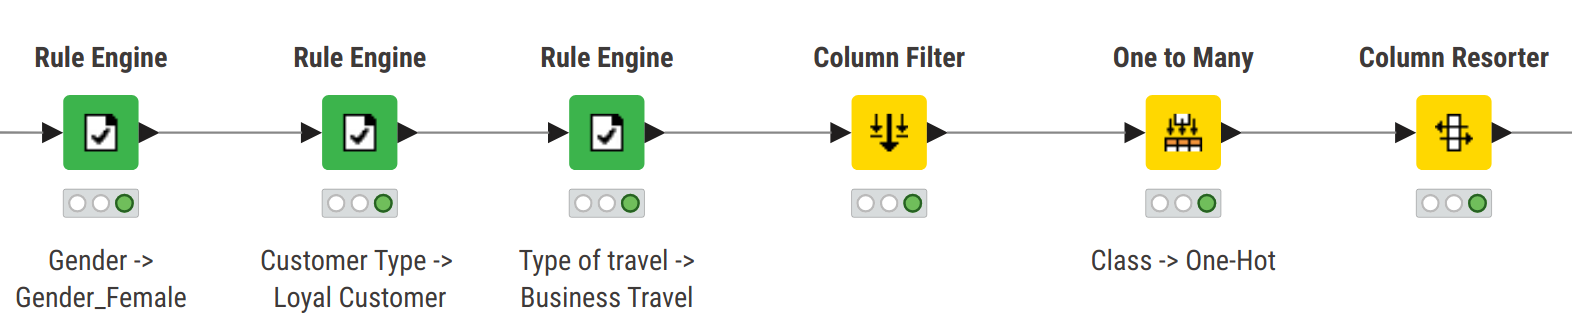
\includegraphics[width=\textwidth, keepaspectratio]{secciones/sec3/imagenes/passenger_satisfaction_categorical_encoding.png}}
    \caption{
        Codificación de los atributos categóricos.
    }
    \label{fig:passenger_satisfaction_categorical_encoding}
\end{figure} 

% ---------------------------------------------------------------------------------------------------------- %

\subsubsection{Imputación de valores faltantes}

Entre todos los atributos, el único que presenta valores faltantes es \code{Arrival Delay}. Para abordar esta situación, se ha creado un imputador basado en un modelo predictivo de \textit{Gradient Boosting} que estima los valores faltantes de retraso a la llegada a partir de los siguientes atributos: \code{Flight Distance} y \code{Departure Delay in Minutes}. 

Se ha decidido utilizar únicamente estos dos atributos porque son los más directamente relacionados con la variable a imputar, reflejando tanto la duración esperada del vuelo (si bien en el análisis se observaba una correlación nula entre la distancia de vuelo y los retrasos) como el retraso acumulado desde el despegue. No se han incluido variables de valoración del servicio, ya que no guardan una relación causal ni temporal con los retrasos, y su inclusión podría introducir ruido o sesgos en el proceso de imputación.

Dado que el modelo de imputación se ajusta a los datos de entrenamiento, es esencial entrenarlo únicamente con las filas que tienen valores conocidos de retraso a en el conjunto de entrenamiento, evitando el uso de cualquier dato del conjunto de test. Esto se hace para mantener la integridad del modelo y prevenir la filtración de información del conjunto de test hacia el entrenamiento. Si el modelo se entrenara con filas del conjunto de test, podría aprender patrones específicos de este, generando un sesgo que influiría en las métricas de evaluación y comprometería la validez del proceso de validación. La Figura \ref{fig:passenger_satisfaction_imputer_arrival_delay} muestra el esquema final. 

\begin{figure}[h!]
    \centering
    \fbox{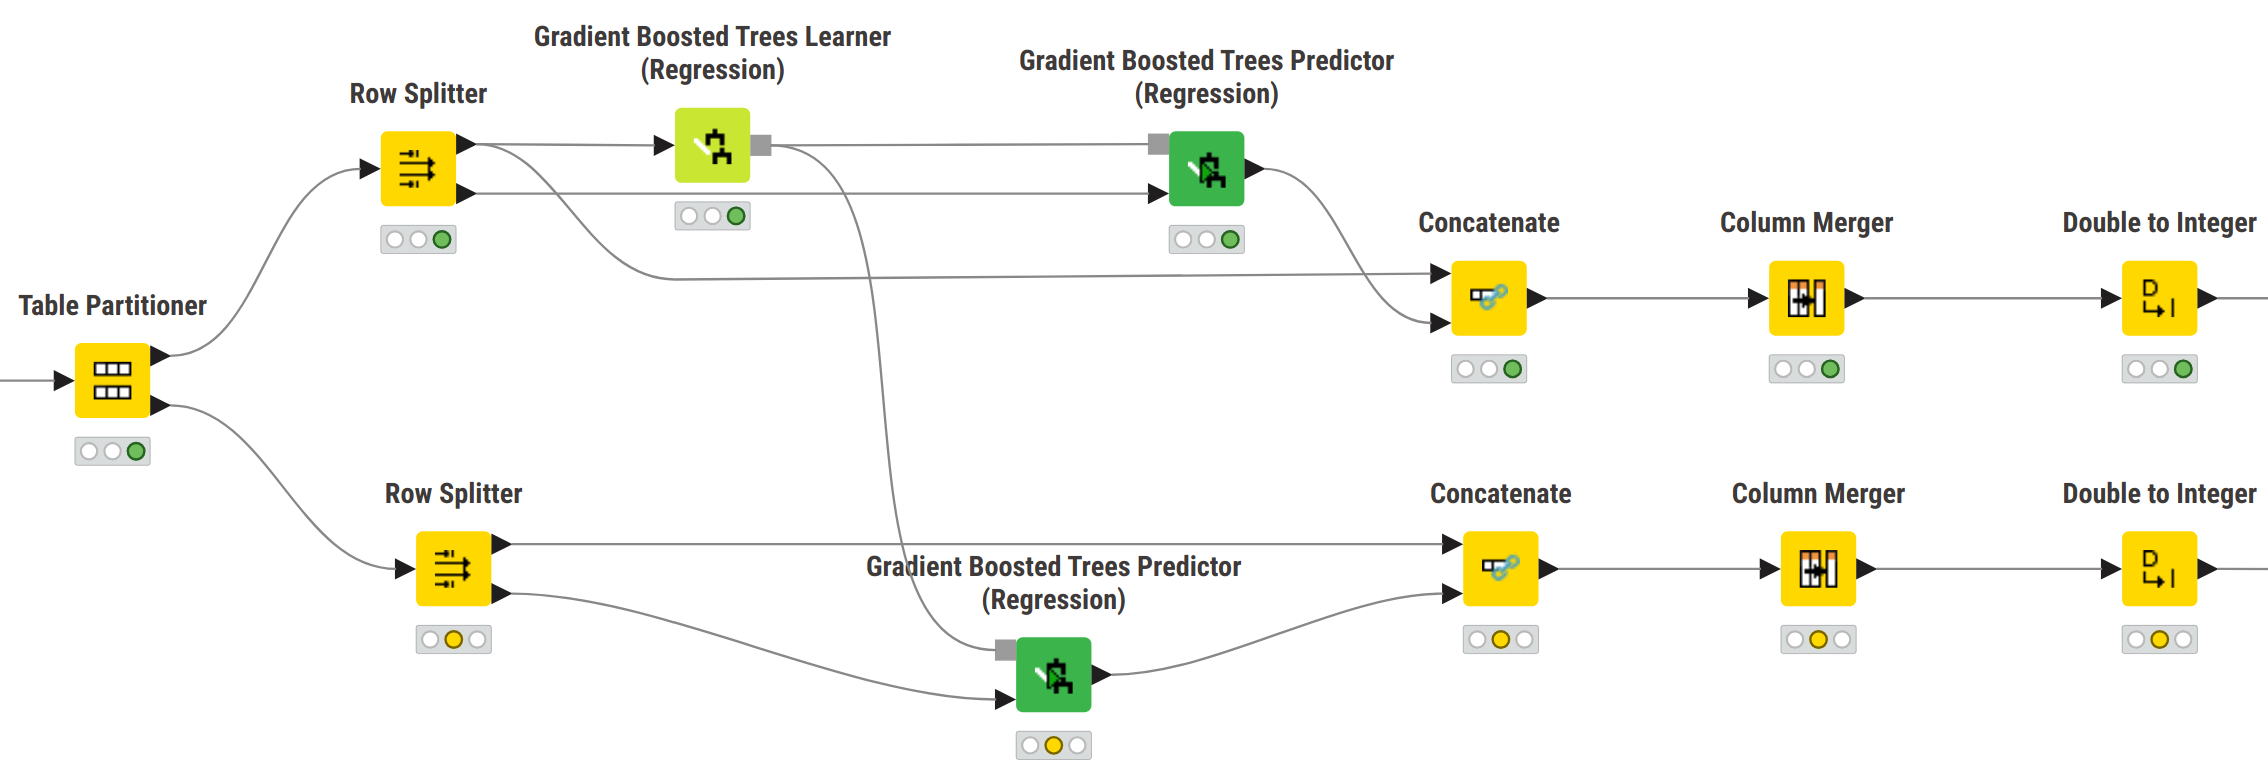
\includegraphics[width=\textwidth, keepaspectratio]{secciones/sec3/imagenes/passenger_satisfaction_imputer_arrival_delay.png}}
    \caption{
        División de datos en entrenamiento y test, e imputación de valores faltantes de \code{Arrival delay in Minutes}.
    }
    \label{fig:passenger_satisfaction_imputer_arrival_delay}
\end{figure} 

% ---------------------------------------------------------------------------------------------------------- %

\subsubsection{Normalización de las variables numéricas}

Como en el anterior problema, una vez todas las variables se han representado como numéricas, se normalizan con Z-Score.

% ---------------------------------------------------------------------------------------------------------- %

\subsubsection{Selección de carísticas}

Dado el alto volumen de datos manejados, se planteó la necesidad de reducir el tamaño y la complejidad del \textit{dataset}, con el objetivo de optimizar el rendimiento computacional y eliminar posibles variables redundantes o irrelevantes.

Para ello, se llevó a cabo un proceso de selección de características mediante los nodos <<Feature Selection Loop>>, utilizando un modelo de regresión logística como estimador base. Este modelo se eligió por su eficiencia computacional y buen desempeño preliminar en las pruebas iniciales, lo que lo convierte en una opción adecuada para identificar las variables más relevantes en la predicción de la satisfacción de los pasajeros.

\begin{figure}[h!]
    \centering
    \fbox{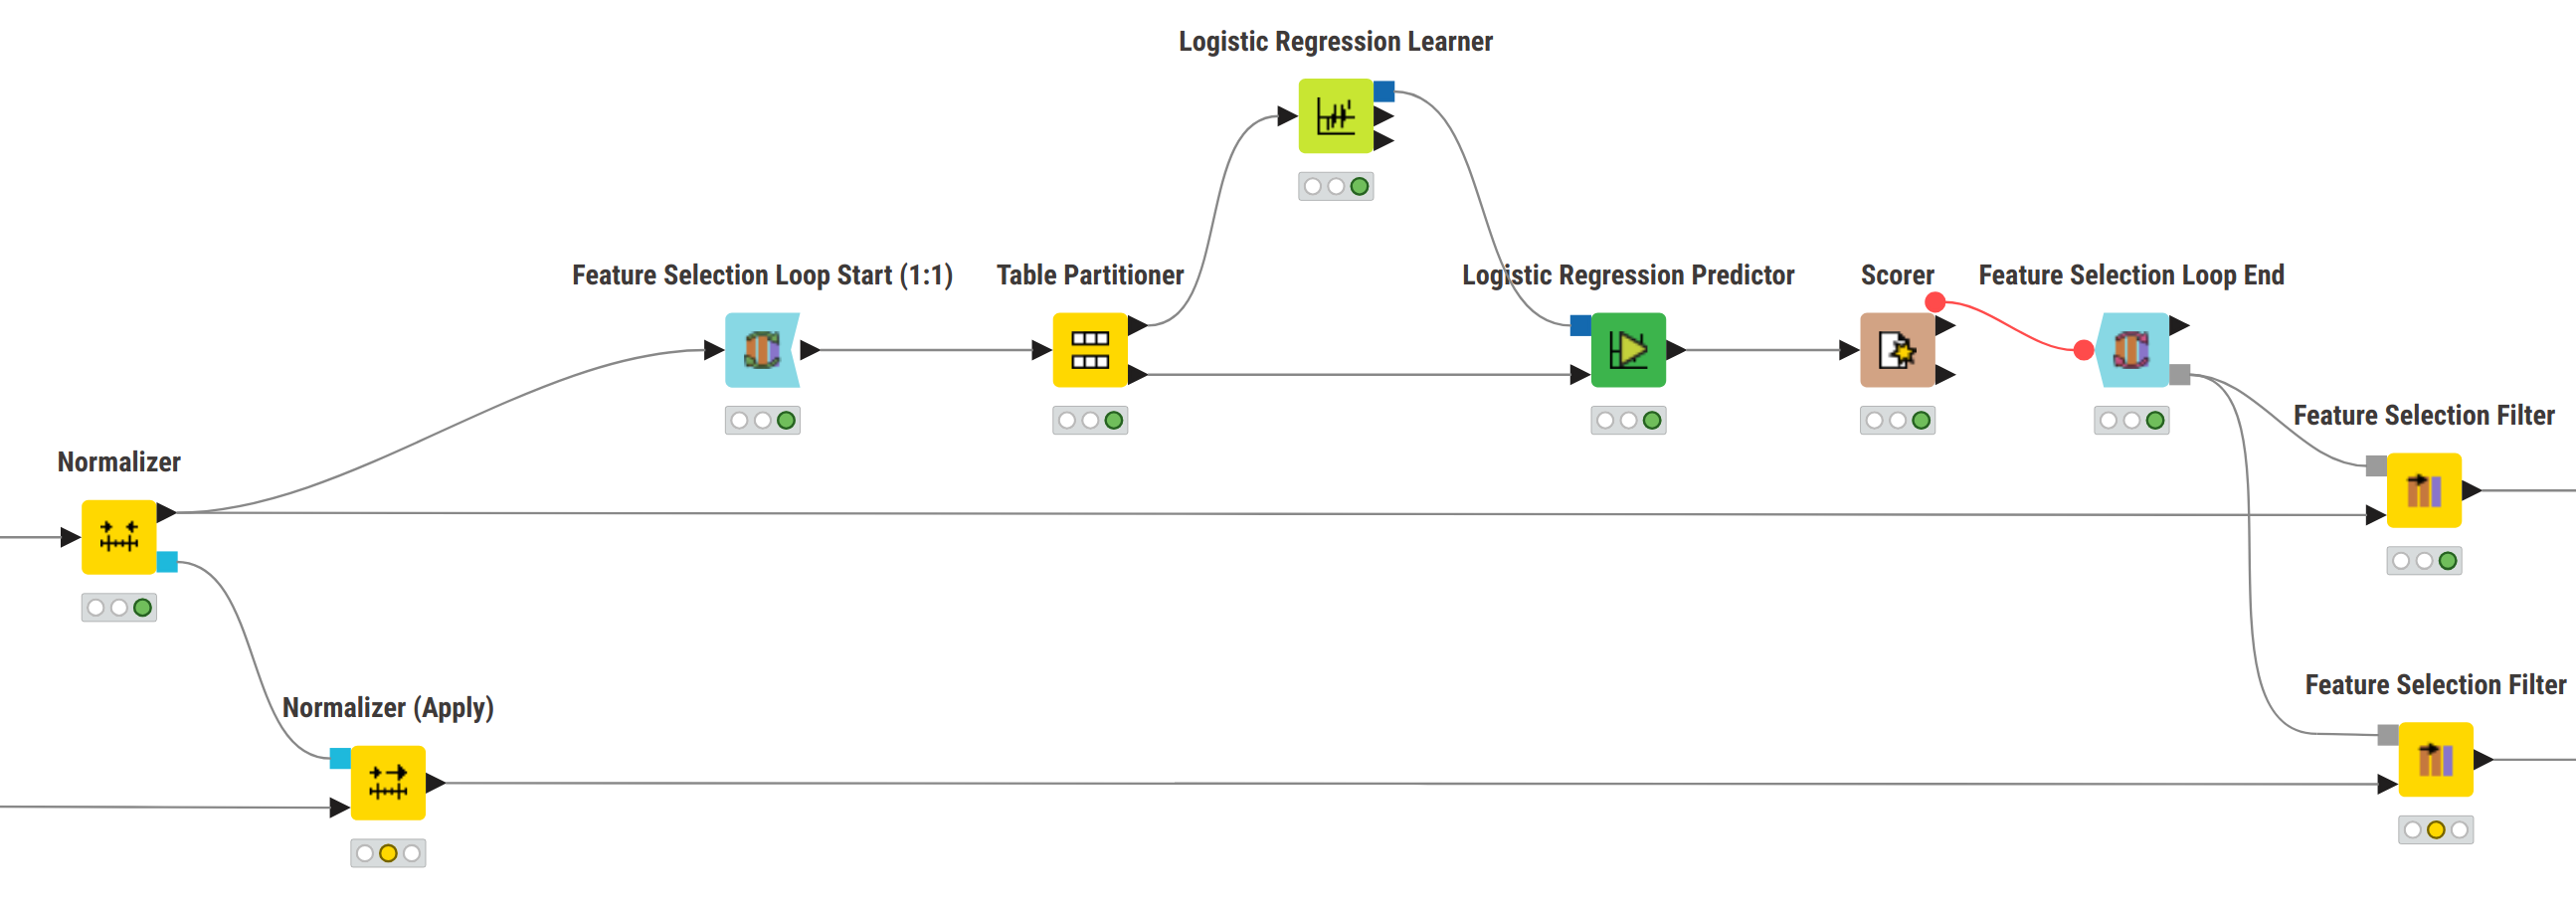
\includegraphics[width=\textwidth, keepaspectratio]{secciones/sec3/imagenes/passenger_satisfaction_normalizer_feature_selection.png}}
    \caption{
        Normalización y selección de características. 
    }
    \label{fig:passenger_satisfaction_normalizer_feature_selection}
\end{figure} 

Se ha escogido el algoritmo genético para escoger las características, con poblaciones de 20 individuos (selecciones de características) durante 10 generaciones con \textit{accuracy} como métrica a maximizar. Finalmente, se logra la mejor marca (86.9\% de \textit{accuracy}) descartando los siguientes atributos: \code{Departure/Arrival time convenient}, \code{Seat comfort}, \code{Inflight entertainment}, \code{Cleanliness}, \code{Arrival Delay} y los tres atributos \textit{One-Hot} derivados de \code{Class} (\code{Eco}, \code{Eco Plus} y \code{Business}).

Respecto a \code{Arrival Delay}, tiene sentido, ya que está fuertemente correlacionada con \code{Departure Delay}, como hemos podido ver antes, por lo que es redundante (aunque es una pena para el esfuerzo que se ha hecho antes en la imputación de valores). 

% ---------------------------------------------------------------------------------------------------------- %
% ---------------------------------------------------------------------------------------------------------- %
% ---------------------------------------------------------------------------------------------------------- %

\subsection{Materiales y métodos}

\subsubsection{Modelos escogidos para la comparación}

Se evaluará el rendimiento en los mismos modelos del pasado problema, pero sustituyendo la \textit{Support Vector Machine} por la regresión logística, dado que el SVM tardaba mucho en entrenar, especialmente cuando usa un kernel polinómico de varios grados. Y en este problema se tiene un volumen de datos significativamente mayor. 

\begin{itemize}
    \item \textbf{Logistic Regression}: Este modelo tiene mucha fundamentación estadística, es usado para resolver problemas de clasificación binaria. La regresión logística modela la probabilidad de que la variable objetivo sea la clase positiva dado un conjunto de variables independientes (los atributos):
    
    $$
    P(y = 1 \mid \mathbf{x}) = \frac{1}{1 + e^{-(\beta_0 + \beta_1 x_1 + \beta_2 x_2 + \dots + \beta_p x_p)}}
    $$
    donde:
    \begin{itemize}
        \item $P(y = 1 \mid \mathbf{x})$ es la probabilidad de que la observación pertenezca a la clase positiva.
        \item $\beta_0$ es el término independiente o sesgo (\textit{bias}).
        \item $\beta_i$ son los coeficientes asociados a cada variable independiente $x_i$.
    \end{itemize}

    De manera equivalente, se puede expresar el modelo en su forma \textit{logit}:
    
    $$
    \log\left(\frac{P(y = 1 \mid \mathbf{x})}{1 - P(y = 1 \mid \mathbf{x})}\right)
    = \beta_0 + \beta_1 x_1 + \beta_2 x_2 + \dots + \beta_p x_p
    $$
    
    Esta expresión representa la relación lineal entre los predictores y el \textit{log-odds} (logaritmo de la razón de probabilidades) de pertenecer a la clase positiva.

    El modelo utiliza la función logística (o sigmoide) (véase la Figura \ref{fig:sigmoid}) para mapear una combinación lineal de las variables de entrada (los \textit{log-odds}) a un valor de probabilidad entre 0 y 1.
    
    \begin{figure}[h!]
        \centering
        \fbox{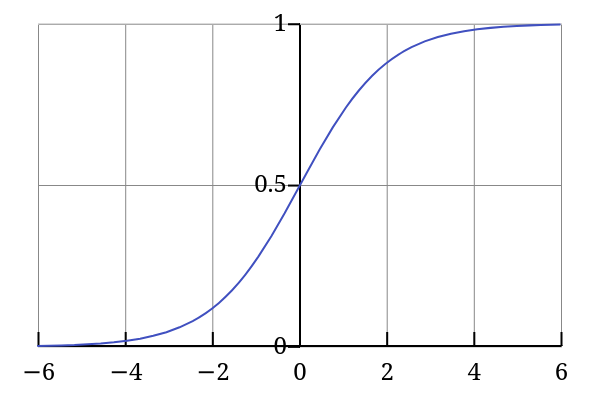
\includegraphics[width=0.5\textwidth, keepaspectratio]{secciones/sec3/imagenes/sigmoid.png}}
        \caption{Función sigmoide. Convierte una combinación lineal en una probabilidad (entre 0 y 1).}
        \label{fig:sigmoid}
    \end{figure}

    Partiendo de esta base, los diferentes algoritmos difieren en cómo calcular los valores beta ($\beta$). 

    En KNIME se implementa mediante el nodo \textit{<<Logistic Regression>>}, que estima los coeficientes del modelo mediante el método de \textbf{máxima verosimilitud} (\textit{Maximum Likelihood Estimation, MLE}). KNIME emplea el algoritmo \textbf{Stochastic Average Gradient (SAG)}. El resultado final son los valores de $\beta$ que maximizan la verosimilitud penalizada, describiendo la relación entre las variables predictoras y la probabilidad de pertenecer a la clase positiva.

\end{itemize}

% ---------------------------------------------------------------------------------------------------------- %

\subsubsection{Métricas escogidas para la evaluación del rendimiento}

Para la evaluación del desempeño de los modelos utilizaremos las mismas métricas que en el problema pasado, ya que este se trata también de una clasificación binaria. 

% ---------------------------------------------------------------------------------------------------------- %
% ---------------------------------------------------------------------------------------------------------- %
% ---------------------------------------------------------------------------------------------------------- %

\subsection{Experimentación}

\subsubsection{Definición del protocolo de validación experimental}

Como en el anterior problema, dividiremos los datos en conjuntos de entrenamiento, validación y \textit{test}.Los datos de \textit{test} no se utilizarán para evaluar el rendimiento del modelo hasta haber escogido y configurado un solo modelo final. Y los datos de validación se obtendrán de las diferentes particiones resultantes de la validación cruzada sobre el conjunto de datos de entrenamiento. Al igual que en el anterior problema, se realizará un \textit{k-fold} con $k$ = 5.

% ---------------------------------------------------------------------------------------------------------- %

\subsubsection{Optimización de hiperparámetros}

Se ha realizado el mismo proceso de optimización de hiperparámetros que en el anterior problema. Las configuraciones óptimas obtenidas para cada modelo fueron las siguientes:

\begin{itemize}
    \item Modelo \textit{k}-NN con $k=7$.
    \item Modelo \textit{Logistic Regression} entrenado mediante el algoritmo \textit{Stochastic Average Gradient} durante 143 iteraciones.
    \item Modelo \textit{Decision Tree} con poda basada en el criterio MDL y un mínimo de 2 instancias por nodo interno.
    \item Modelo \textit{Random Forest} compuesto por 420 árboles, con una profundidad máxima de 512 y un mínimo de 2 instancias por nodo interno.
    \item Modelo \textit{Gradient Boosting} con 284 árboles, una profundidad máxima de 4 y una tasa de aprendizaje (\textit{learning rate}) de 0.25.
\end{itemize}

% ---------------------------------------------------------------------------------------------------------- %

\subsubsection{Comparación de modelos candidatos}

Los modelos candidatos obtuvieron las métricas mostradas en la Figura \ref{fig:passenger_satisfaction_metrics_comparison}. En esta se observa marcas muy superiores a las vistas en el anterior problema: en este sí se consiguen buenos predictores, logrando todos G-Mean superior a $0.85$. Aun así, los modelos \textit{ensemble} (\textit{Random Forest} y \textit{Gradient Boosting}) logran batir todas las marcas del resto de modelos. 

\begin{figure}[h!]
    \centering
    \fbox{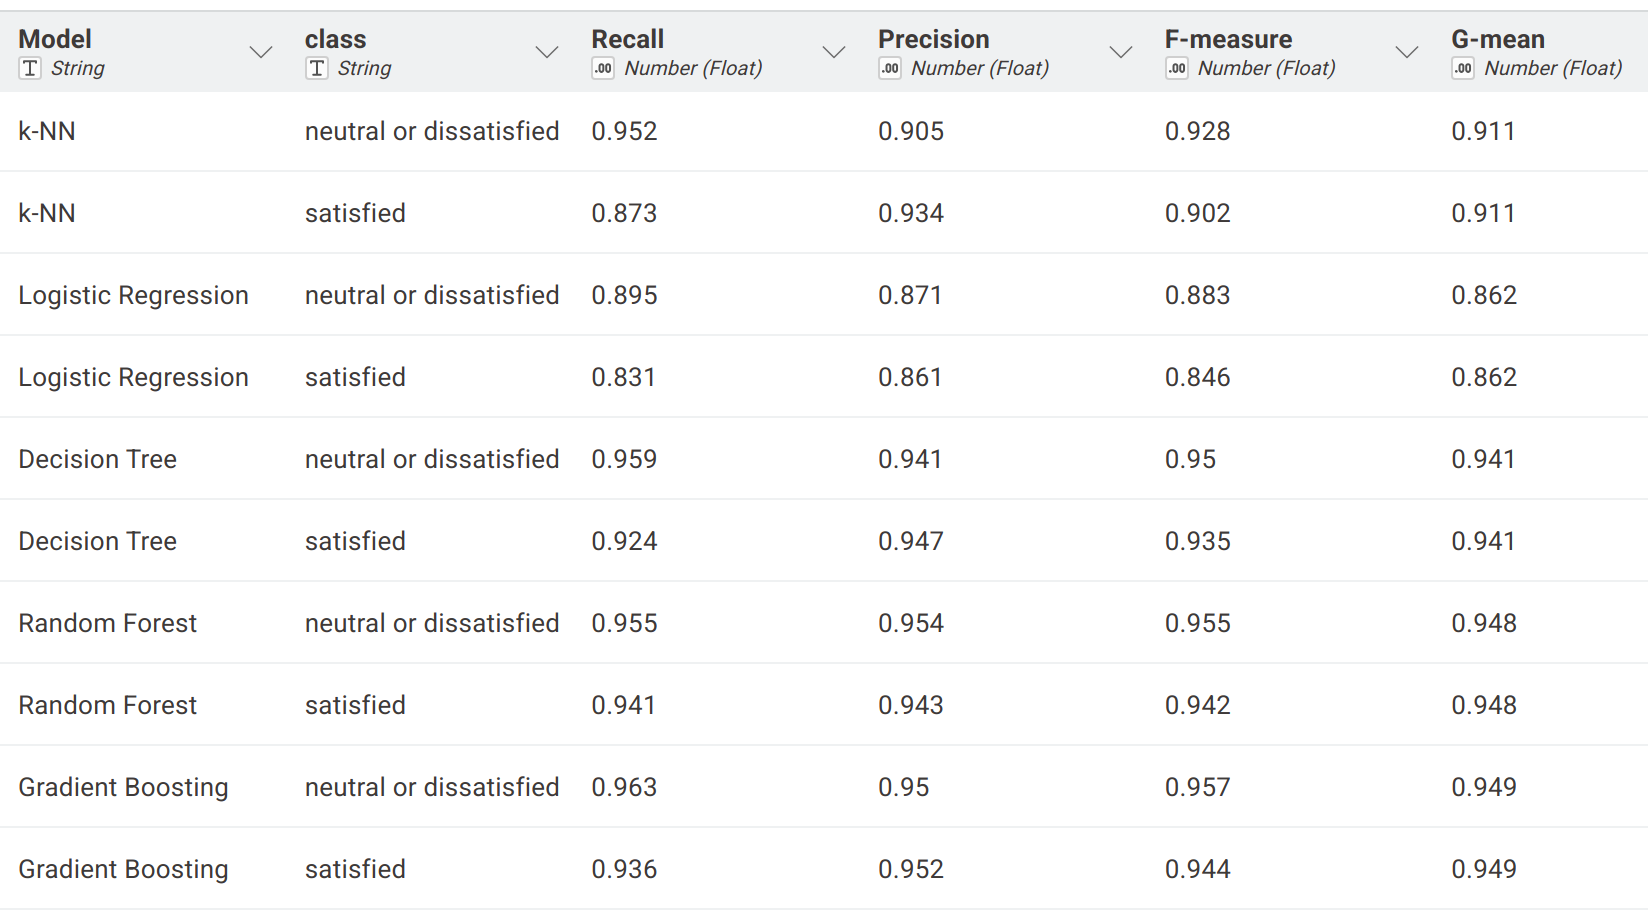
\includegraphics[width=\textwidth, keepaspectratio]{secciones/sec3/imagenes/passenger_satisfaction_metrics_comparison.png}}
    \caption{
        Métricas de desempeño logradas por los modelos candidatos.
    }
    \label{fig:passenger_satisfaction_metrics_comparison}
\end{figure} 

En la Figura \ref{fig:passenger_satisfaction_ROC_comparison} podemos ver cómo las curvas ROC de estos modelos \textit{ensemble} muestra una gran estabilidad, ya que mantiene una forma cóncava pronunciada y se aproxima al vértice superior izquierdo, indicando una alta capacidad de discriminación entre clases. Esta estabilidad refleja cómo los modelos \textit{ensemble} logran reducir la variabilidad y mejorar el rendimiento general al combinar múltiples predictores. El área bajo la curva (AUC) es consistentemente alta, demostrando que estos modelos mantienen una buena tasa de verdaderos positivos (TPR) mientras minimizan los falsos positivos (FPR) en distintos umbrales de decisión.

\begin{figure}[h!]
    \centering
    \fbox{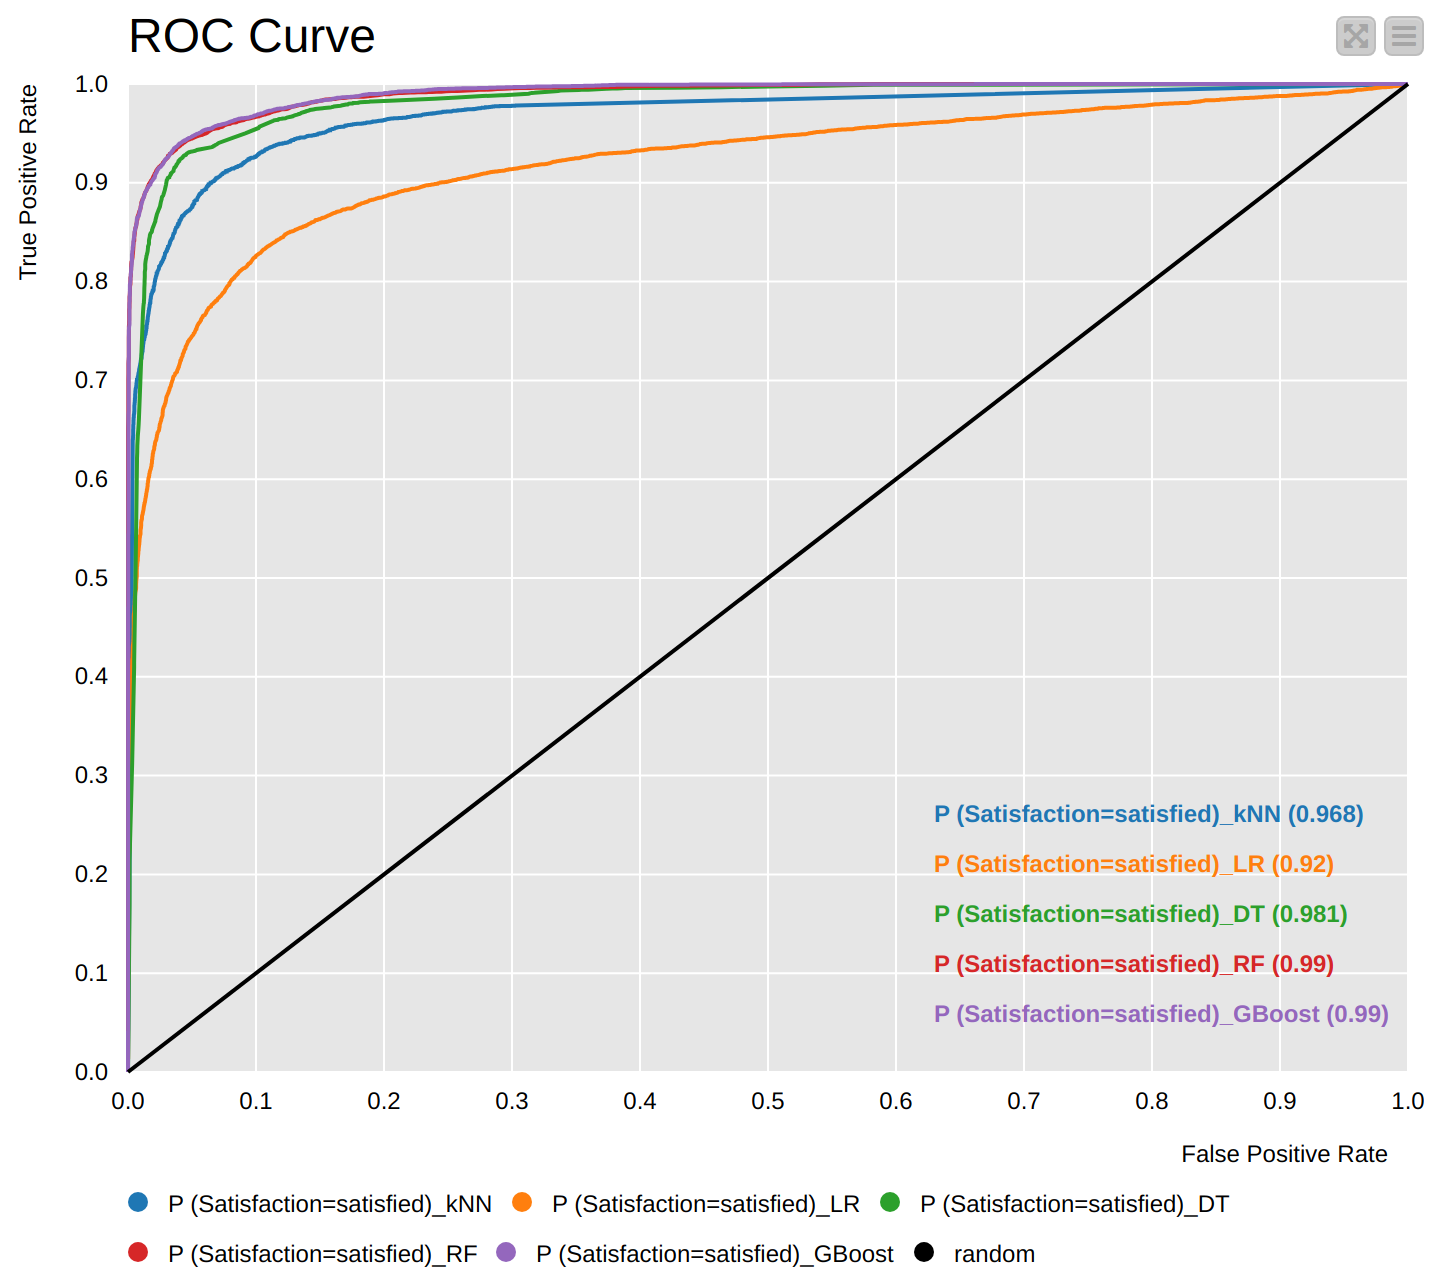
\includegraphics[width=\textwidth, keepaspectratio]{secciones/sec3/imagenes/passenger_satisfaction_ROC_comparison.png}}
    \caption{
        Curvas ROC de los modelos candidatos.
    }
    \label{fig:passenger_satisfaction_ROC_comparison}
\end{figure} 

El modelo de \textit{Gradient Boosting} logra incluso unos resultados superiores a los del \textit{Random Forest}, gracias a que optimiza los errores de manera iterativa. Por tanto, este será nuestro modelo final.

% ---------------------------------------------------------------------------------------------------------- %

\subsubsection{Modelo final}

Entrenamos el modelo final como \textit{Gradient Boosting}, con la misma configuración óptima obtenida en la optimización de hiperparámetros. La Figura \ref{fig:passenger_satisfaction_final_model} muestra el esquema de nodos implementado en KNIME. Este modelo logra resultados muy parejos con los de la comparación previa (véase la Figura \ref{fig:passenger_satisfaction_final_model_metrics}), con F1-Score de $0.948$ para la clase positiva y $0.96$ para la negativa, y un G-Mean de $0.953$, lo que indica una elevada estabilidad y un equilibrio sólido entre la sensibilidad y la especificidad. Estos resultados confirman la consistencia del modelo y su capacidad generalizadora, manteniendo un rendimiento robusto incluso tras los ajustes finales y la reducción de características.

\begin{figure}[h!]
    \centering
    \fbox{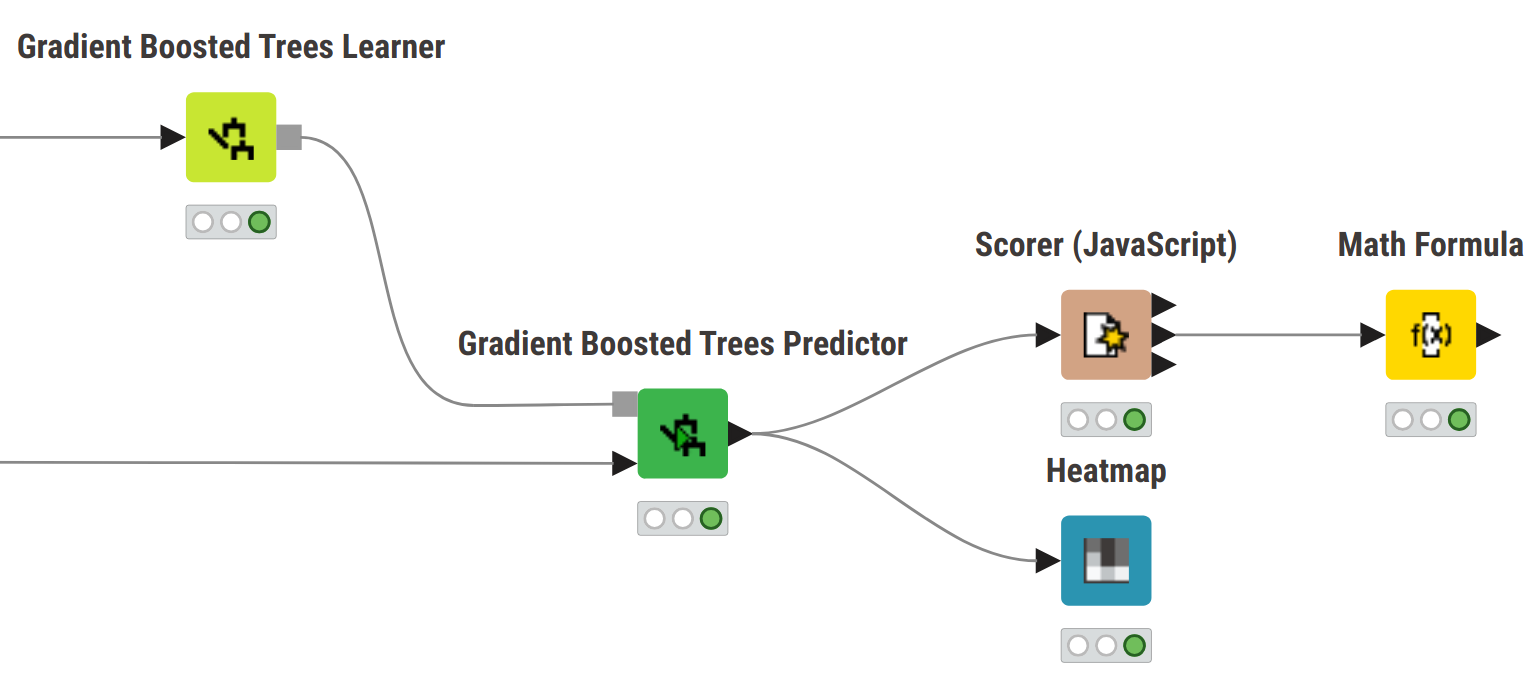
\includegraphics[width=0.65\textwidth, keepaspectratio]{secciones/sec3/imagenes/passenger_satisfaction_final_model.png}}
    \caption{
        Esquema de entrenamiento e inferencia del modelo final. 
    }
    \label{fig:passenger_satisfaction_final_model}
\end{figure} 

\begin{figure}[h!]
    \centering
    \fbox{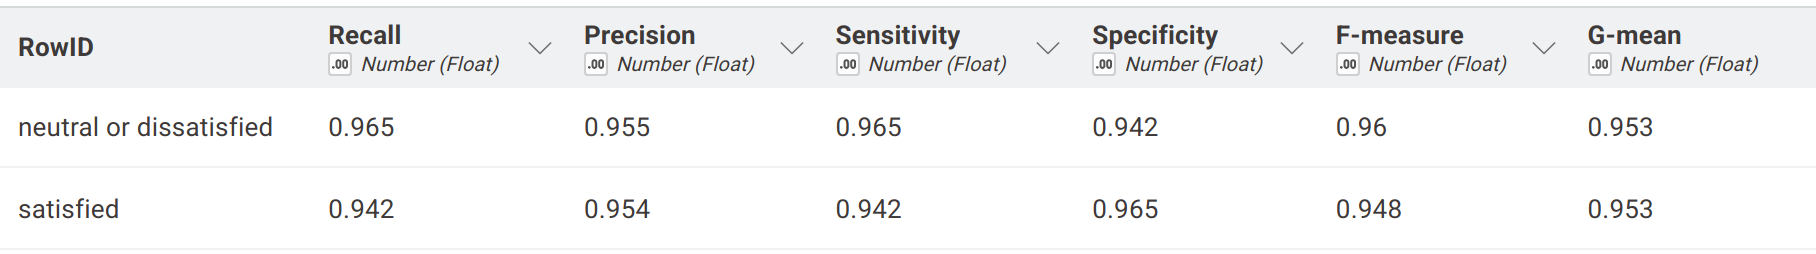
\includegraphics[width=\textwidth, keepaspectratio]{secciones/sec3/imagenes/passenger_satisfaction_final_model_metrics.png}}
    \caption{
        Métricas obtenidas por el modelo final. 
    }
    \label{fig:passenger_satisfaction_final_model_metrics}
\end{figure} 

% ---------------------------------------------------------------------------------------------------------- %

\subsubsection{Estudio adicional de características relevantes}

Dado que el modelo final obtenido es \textit{ensemble}, este es dificilmente interpretrable. Por ello, se realizará un estudio de importancia de características, mediante dos componentes: <<AutoML>> y <<Global Feature Importance>>, del siguiente \textit{workflow} de KNIME: \url{https://hub.knime.com/s/VEfBibUV0gNF_HmB}. 

Primero, se debe especificar un modelo en <<AutoML>>, \textit{Gradient Boosting} en nuestro caso, que logra un F1-Score de 0.928 en la clase positiva, ligeramente inferior a los resultados logrados antes.

La importancia de un atributo no tiene una definición única ni estricta, ya que los modelos de aprendizaje automático aprenden patrones complejos y no lineales entre las variables, los cuales difícilmente pueden interpretarse de una forma directa o aislada. En muchos casos, la contribución de un atributo depende del contexto generado por las demás, lo que hace que su relevancia varíe según las interacciones presentes en el modelo. De hecho, muchas veces se da la paradoja de que aquellos atributos más intuitivas o aparentemente determinantes no resultan ser las más influyentes en el modelo final, mientras que otras variables menos evidentes pueden adquirir una gran importancia al capturar relaciones sutiles o efectos combinados con otras.

Aun así, el componente <<Global Feature Importance>> plantea varias pruebas:

\begin{tcolorbox}
    [colback=gray!5!white, colframe=gray!60!black, title=NOTA, breakable]

    Por falta de tiempo, no se entra más en detalle de cómo se realiza cada una de las pruebas.

\end{tcolorbox}

\begin{itemize}
    
    \item \textbf{Surrogate Generalized Linear Model}: Este modelo trata de aproximar las predicciones del modelo original (el especificado en <<AutoML>>) mediante una relación lineal entre las variables explicativas y la variable objetivo. Su principal ventaja es la interpretabilidad: permite entender cómo cada variable contribuye positiva o negativamente a la probabilidad de que un pasajero esté satisfecho. De esta forma, el GLM actúa como un modelo sustituto que explica, de manera simplificada, el comportamiento global del modelo complejo original.
    
    \begin{tcolorbox}
        [colback=gray!5!white, colframe=gray!60!black, title=Interpretación de GML, breakable]

        Este texto ha sido directamente traducido de la visualiación del nodo <<Global Feature Importance>>:

        ``La magnitud del coeficiente GML indica la importancia de la característica: un valor positivo (negativo) significa que un valor mayor conduce a una mayor (menor) probabilidad del evento positivo (\textit{satisfied}).''

    \end{tcolorbox}

    Los resultados obtenidos, mostrados en la Figura \ref{fig:passenger_satisfaction_feature_importance_GLM}, indican que los atributos \code{Online boarding}, \code{Business travel} y \code{Inflight wifi service} son los que más contribuyen a aumentar la satisfacción de los pasajeros. En cambio, \code{Departure Delay} y, sorprendentemente, \code{Ease of Online Booking} aparecen como los que más influyen negativamente, es decir, aquellos asociados con una mayor probabilidad de insatisfacción.

    Este último resultado podría deberse a que la percepción de facilidad en la reserva no necesariamente se traduce en una mejor experiencia global del vuelo, o a que los pasajeros con altas expectativas (que valoran más la facilidad de reserva) tienden a ser más críticos con el servicio en general.
    
    \begin{figure}[h!]
        \centering
        \fbox{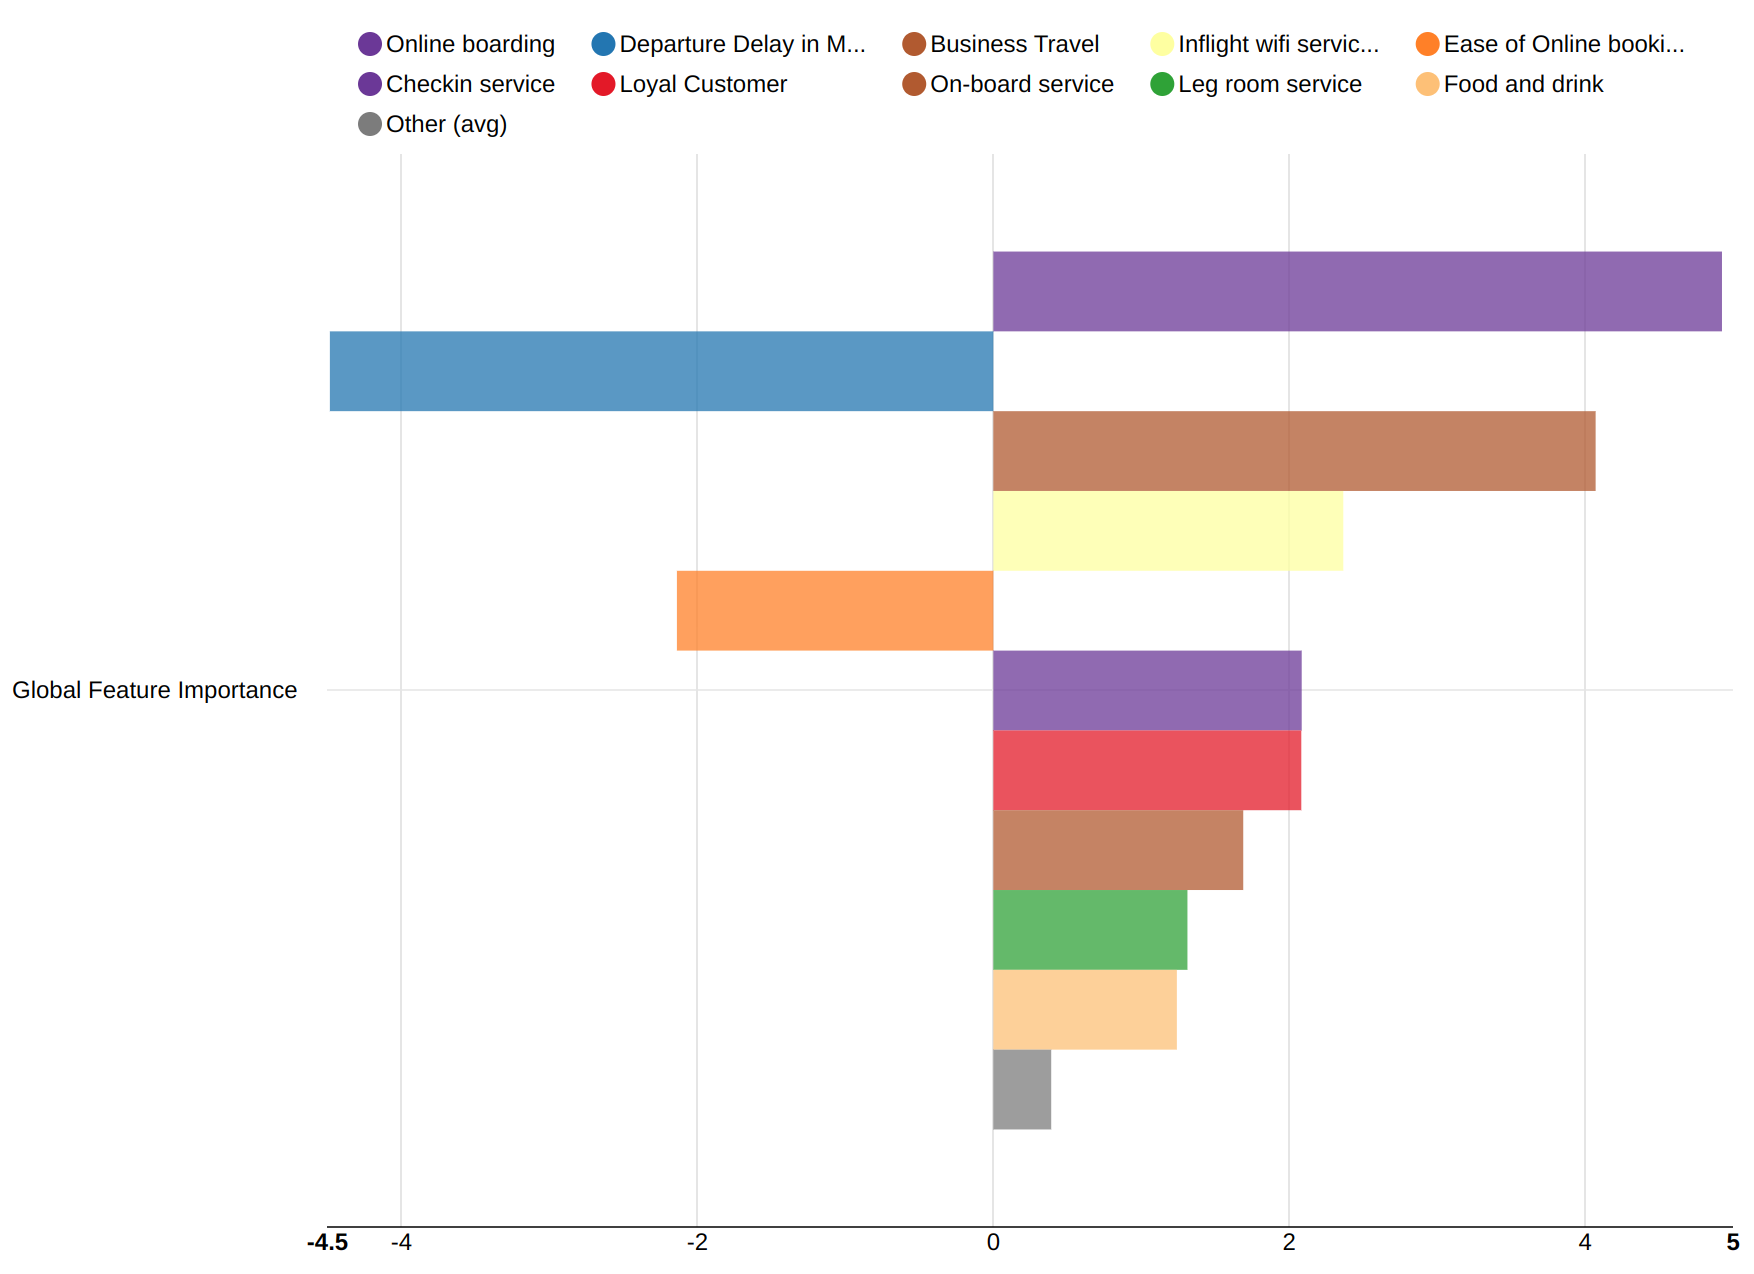
\includegraphics[width=\textwidth, keepaspectratio]{secciones/sec3/imagenes/passenger_satisfaction_feature_importance_GLM.png}}
        \caption{
            Resultados del análisis \textit{Surrogate Generalized Linear Model}.
        }
        \label{fig:passenger_satisfaction_feature_importance_GLM}
    \end{figure} 

    
    \item \textbf{Surrogate Random Forest}: <Explicar en qué consiste>
    
    Este modelo mide la importancia como el número de veces que tiene que seleccionar un determinado atributo para dividir un nodo. Por tanto, un valor mayor indica una importancia mayor.

    Los resultados obtenidos en la Figura \ref{fig:passenger_satisfaction_feature_importance_SRF} indican que los atributos más relevantes son \code{Inflight wifi service}, \code{Online boarding}, \code{Business Travel}, \code{Flight Distance} y \code{Leg room service}. 

    \begin{figure}[h!]
        \centering
        \fbox{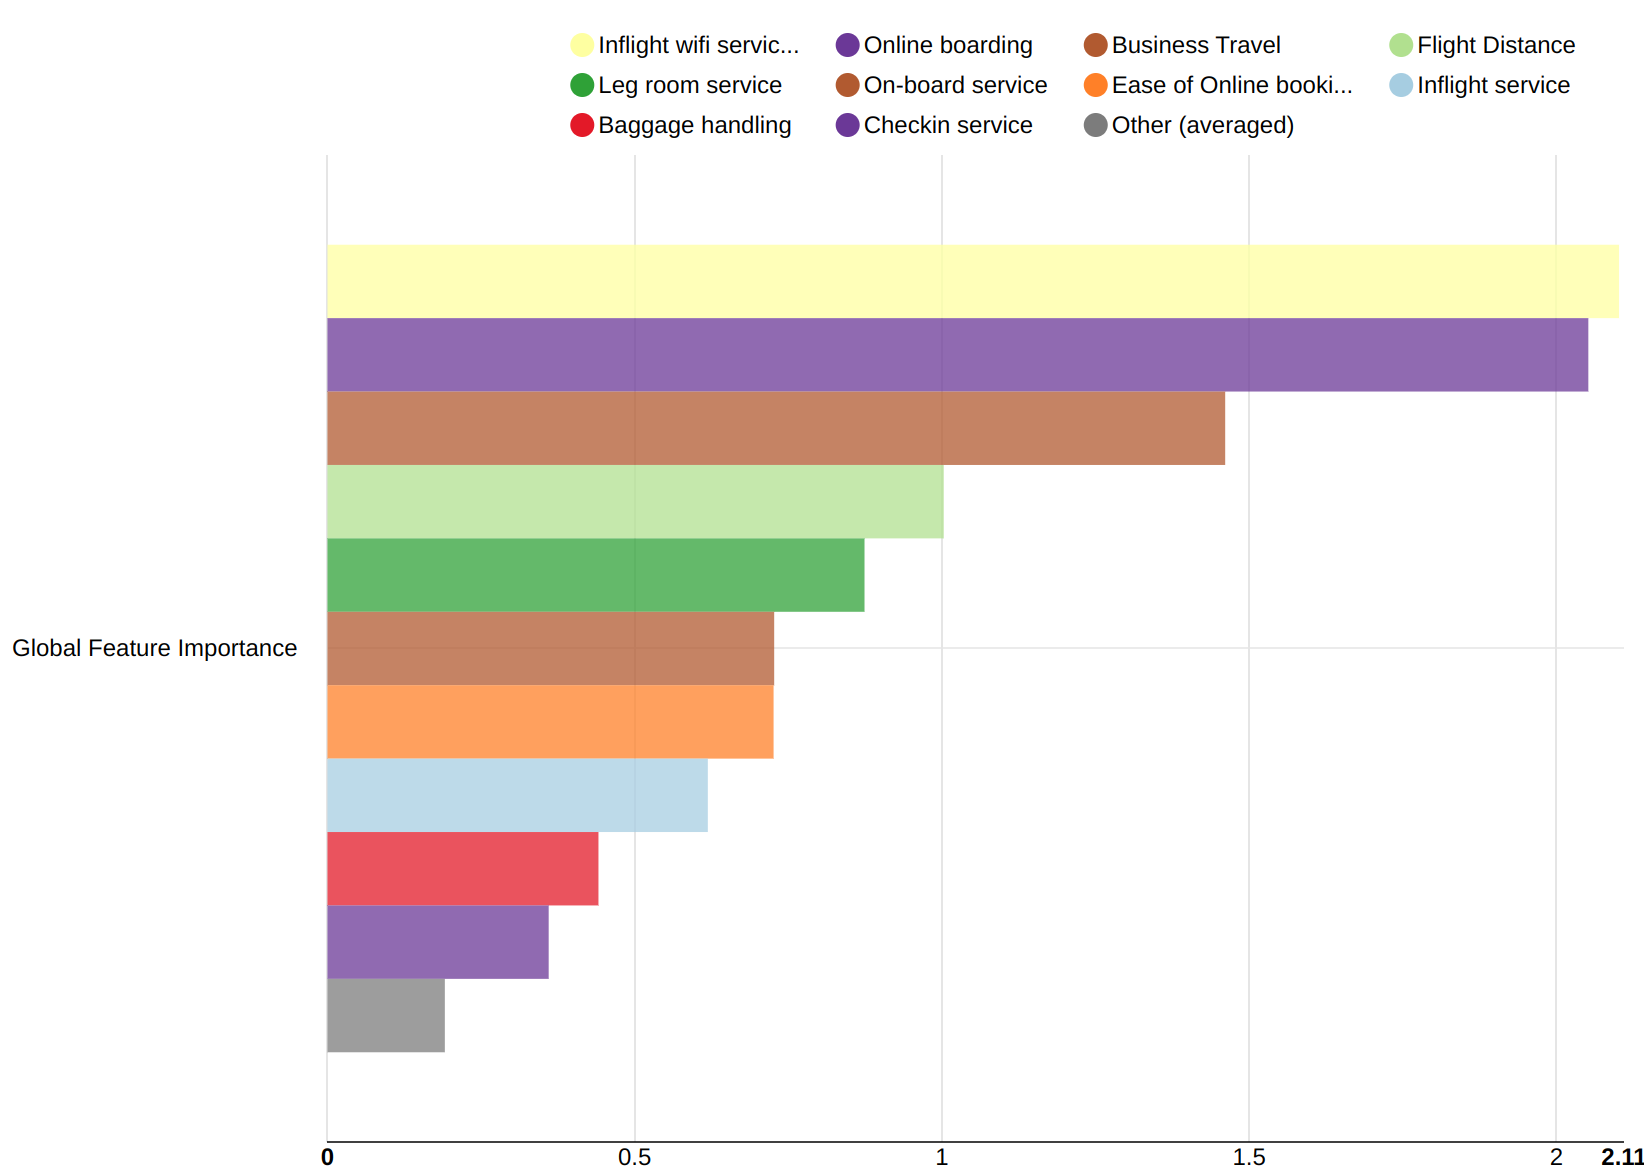
\includegraphics[width=\textwidth, keepaspectratio]{secciones/sec3/imagenes/passenger_satisfaction_feature_importance_SRF.png}}
        \caption{
            Resultados del análisis \textit{Surrogate Random Forest}.
        }
        \label{fig:passenger_satisfaction_feature_importance_SRF}
    \end{figure} 
    

    \item \textbf{Permutation Feature Importance}:Este método evalúa la importancia de cada característica midiendo cuánto empeora el rendimiento del modelo cuando los valores de dicha característica se permutan aleatoriamente, rompiendo así su relación con la variable objetivo. Es decir, compara la puntuación de desempeño del modelo original con la obtenida tras alterar una variable, manteniendo las demás intactas. Si una característica es relevante para las predicciones, al permutarla se producirá una disminución notable en el rendimiento del modelo.
    
    Un \textit{score} alto indica que la variable tiene una gran influencia en la capacidad predictiva del modelo (es decir, que al permutarla el rendimiento se degrada significativamente), mientras que valores cercanos a cero indican baja relevancia.

    Los resultados obtenidos (Figura \ref{fig:passenger_satisfaction_feature_importance_PFI}) indican como más relevantes los siguientes atributos: \code{Business travel},  \code{Inflight wifi service}, \code{Loyal Customer}, \code{Online boarding} y \code{Checkin service}.
    
    \begin{figure}[h!]
        \centering
        \fbox{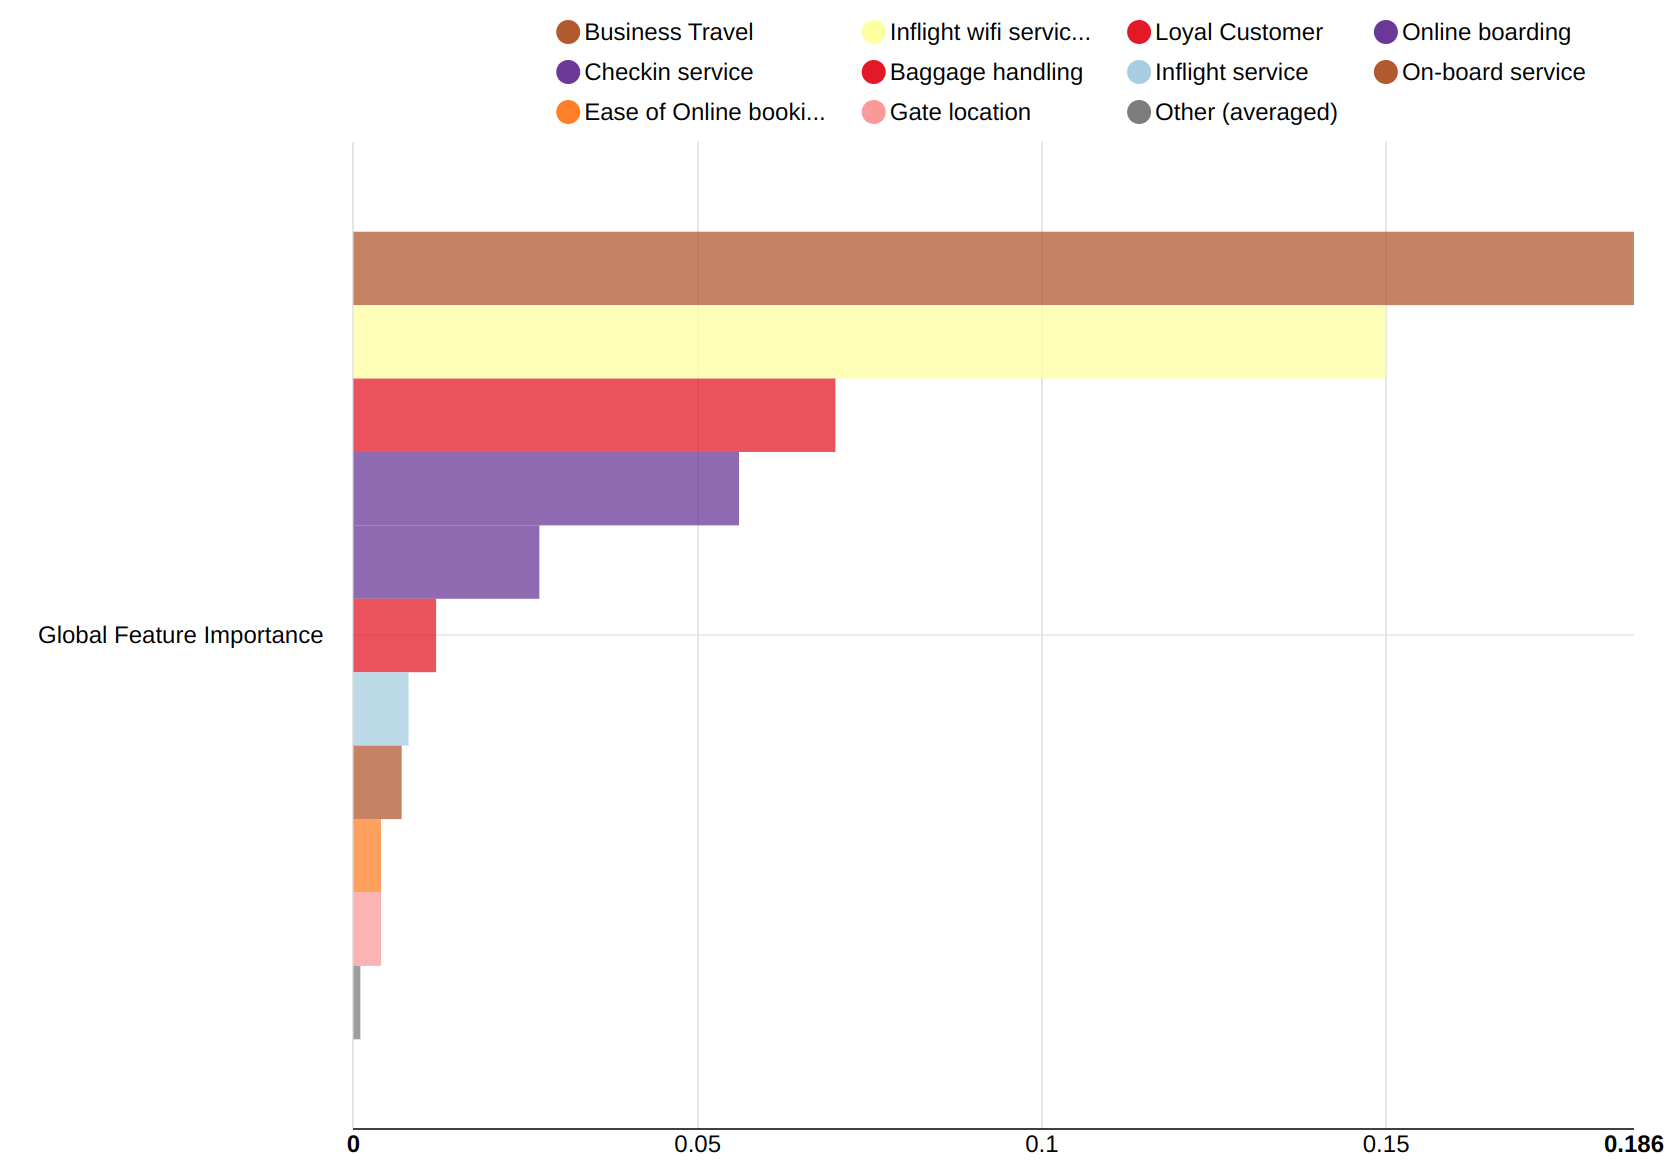
\includegraphics[width=\textwidth, keepaspectratio]{secciones/sec3/imagenes/passenger_satisfaction_feature_importance_PFI.png}}
        \caption{
            Resultados del análisis \textit{Permutation Feature Importance}.
        }
        \label{fig:passenger_satisfaction_feature_importance_PFI}
    \end{figure} 

\end{itemize}

Todas estas pruebas miden aspectos diferentes de la importancia de las características, ya que cada método evalúa la contribución de las variables desde una perspectiva distinta. Sin embargo, los resultados son consistentes entre sí: en todas las pruebas aparecen de forma recurrente entre los primeros puestos las características \code{Business travel}, \code{Online boarding} y \code{Inflight wifi service}. Esto sugiere que dichos atributos tienen una influencia decisiva y robusta en la predicción de la satisfacción de los pasajeros.

% ---------------------------------------------------------------------------------------------------------- %
% ---------------------------------------------------------------------------------------------------------- %
% ---------------------------------------------------------------------------------------------------------- %

\subsection{Conclusión}

Los buenos resultados logrados en este problema demuestran que, a diferencia del anterior, este conjunto de datos sí contiene atributos con un alto poder predictivo respecto a la variable objetivo. Desde el análisis exploratorio ya se observaba que existían variables con una clara capacidad discriminativa entre los pasajeros satisfechos y los insatisfechos, lo cual se ha confirmado posteriormente con los resultados de los modelos.

El mejor modelo, basado en \textit{Gradient Boosting}, alcanza valores de F1-Score y G-Mean superiores al 95\%, evidenciando un excelente equilibrio entre sensibilidad y especificidad, así como una gran capacidad para generalizar a nuevos datos.

Además, se ha podido comprobar que el hecho de que el pasajero viaje por negocios, valore positivamente el embarque en línea y disponga de un buen servicio de WiFi a bordo son los factores que más contribuyen a aumentar la probabilidad de satisfacción.
